\documentclass[usenames,dvipsnames]{beamer}
\usetheme{uhh}
\showtotalframenumber
\showuhhlogoeachframe
\showsections

\usepackage{booktabs}
\usepackage{xcolor}
%\usepackage{amsmath}
\usepackage{graphicx}
\usepackage{color}
\usepackage{algorithm}
\usepackage[noend]{algorithmic}
\usepackage{amsmath,amsfonts,amssymb}
\usepackage{animate}

\usefonttheme{professionalfonts}

\renewcommand{\algorithmicrequire}{\textbf{Input:}}
\newcommand{\REQUIREP}{\item[\hphantom{\textbf{Input:}}]}
\renewcommand{\algorithmicensure}{\textbf{Output:}}

\DeclareMathOperator*{\argmin}{arg\,min}


\DeclareMathOperator{\NN}{\mathrm{NN}}
\DeclareMathOperator{\ctx}{\mathrm{ctx}}
\DeclareMathOperator{\ssim}{\mathrm{sim}}
\DeclareMathOperator{\tfidf}{\mathrm{tf}--\mathrm{idf}}
\DeclareMathOperator{\nmpu}{\mathrm{nmPU}}
\DeclareMathOperator{\nipu}{\mathrm{niPU}}

\newcommand{\watset}{\textsc{Watset}}


\newcommand\legend[1]{\fcolorbox{white}{#1}{\rule{0pt}{6pt}\rule{6pt}{0pt}}}
\definecolor{ggplotverb}{HTML}{b2abd2}
\definecolor{ggplotsubject}{HTML}{e66101}
\definecolor{ggplotobject}{HTML}{fdb863}
\definecolor{ggplotframe}{HTML}{5e3c99}


\usepackage{listings}
\lstset{
  language=python
  }

\title[From unsupervised induction of linguistic
structures to applications in deep learning]{From unsupervised induction of linguistic
structures from text towards applications in deep learning}

\author[A. Panchenko]{Alexander Panchenko} 
\date[28.05.2018]{May 28, 2018}

\AtBeginSection[]
{
   %%%%% section title
   % This is how it would look like in Beamer:
   % \begin{frame}
   %     \frametitle{Overview}
   %     \tableofcontents[sections={2-3},currentsection,sectionstyle=show/hide,subsectionstyle=hide]
   % \end{frame}
  \begin{frame}[plain]
  \begin{tikzpicture}[overlay]
    \relax%
    \fill[blueuhh,opacity=1] (-10,-10)
    rectangle(\the\paperwidth,\the\paperheight);
  \end{tikzpicture}
   \begin{tikzpicture}[overlay]
    \relax%
    \fill[white,opacity=1] (-5,-1.2)
    rectangle(\the\paperwidth,0.5) node[pos=0.5,black]{\LARGE\insertsectionhead};
  \end{tikzpicture}
  \end{frame}

  %%%% add subsection to show navigation dots
  \subsection{}
}


\begin{document}


\maketitle


\begin{frame}
  \frametitle{In close collaboration with ... }

 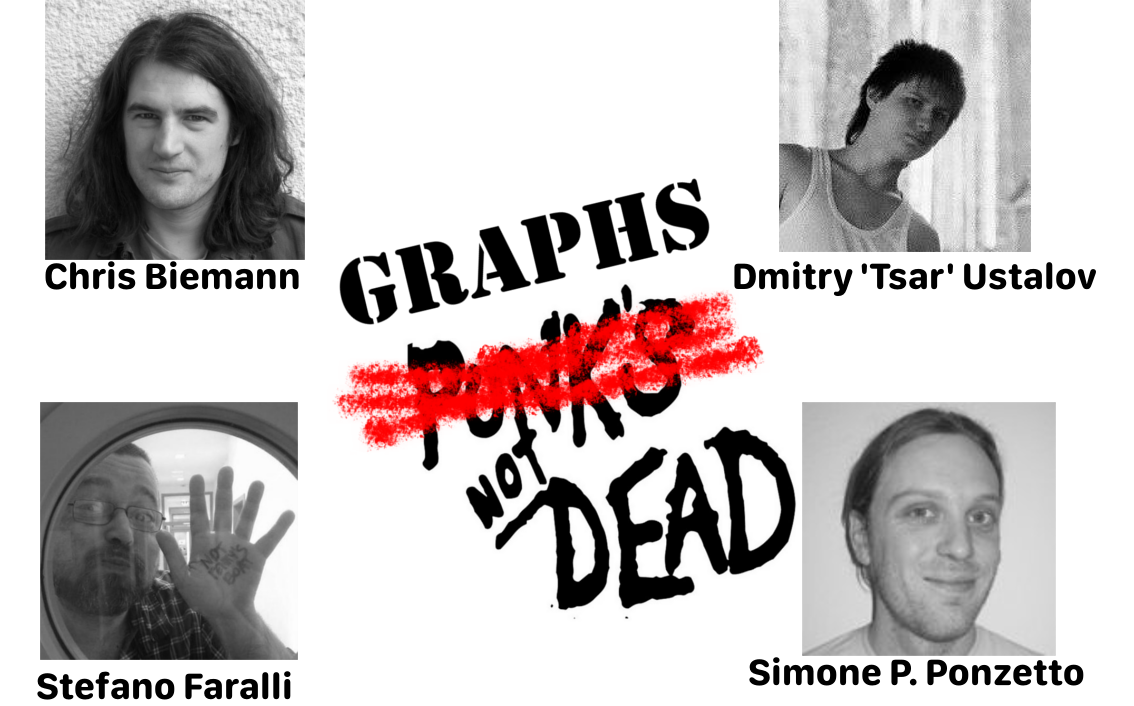
\includegraphics[width=.95\textwidth]{figures/collaborators}	
\end{frame}



\begin{frame}
  \frametitle{In collaboration with ... }
  { \large \bf
  \begin{itemize}
  	\item Andrei Kutuzov
  	\item Eugen Ruppert
  	\item Fide Marten
  	\item Nikolay Arefyev
  	\item Steffen Remus
  	\item Martin Riedl
  	\item Hubert Naets
   	\item Maria Pelevina
	\item Anastasiya Lopukhina
	\item Konstantin Lopukhin
  
  \end{itemize}	
  }
\end{frame}


\section{Overview}

\begin{frame}
  \frametitle{Overview}

  \begin{itemize}
		\item \alert{\textbf{Inducing word sense representations}}:
		\begin{itemize}
		\item \textbf{word sense embeddings via retrofitting} \cite{pelevina-EtAl:2016:RepL4NLP,remus:2018};
		\item \textbf{inducing synsets}~\cite{ustalov-panchenko-biemann:2017:Long,ustalov2017fighting,madoc43362}
		\item \textbf{inducing semantic classes} \cite{panchenko:2018:SemanticClasses} 
				
		\end{itemize}

	
	\pause 
	\vspace{1em}
	\item \alert{\textbf{Making induced senses interpretable}} \cite{panchenko-EtAl:2017:EMNLP2017Demos,panchenko-EtAl:2017:EACLlong}
	
	\pause
	\vspace{1em}
	\item \alert{\textbf{Linking induced word senses to lexical resources}}~\cite{panchenko2016best,faralli2016linked,panchenko-EtAl:2017:SENSE2017,biemann2018framework}	
			
\end{itemize}
	
\end{frame}


\begin{frame}
  \frametitle{Overview}

  \begin{itemize}
  
  			\item \alert{\textbf{A shared task on word sense induction}} \cite{panchenko2018russe,arefyev2018russe}	
  		
  		\pause 	
  		\vspace{10pt}
  
		\item \alert{\textbf{Inducing semantic frames}} \cite{ustalov2018unsupervised} 
		\begin{itemize}
			\item Inducing \textbf{FrameNet}-like structures;
			\item ...using \textbf{multi-way clustering}.
		\end{itemize}
		
		\pause 
		\vspace{10pt} 
		
		\item \alert{\textbf{Learning graph/network embeddings}} [ongoing joint work with Andrei Kutuzov and Chris Biemann]
		\begin{itemize}
		\item How to \textbf{represent induced networks/graphs}?
		\item ... so that they can be used in \textbf{deep learning architectures}.
		\item ...\textbf{effectively} and \textbf{efficiently}.
		\end{itemize}
		
		 
				
	
			
\end{itemize}
	
\end{frame}





\section{Inducing word sense representations}


\subsection{Related work}

\begin{frame}{Word vs sense embeddings}

\begin{center}
	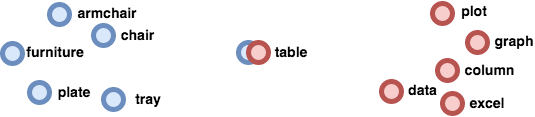
\includegraphics[width=1.0\textwidth]{table-ambigous}
\end{center}	
\end{frame}

\begin{frame}{Word vs sense embeddings}

\begin{center}
	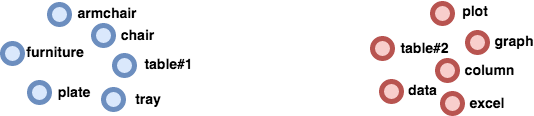
\includegraphics[width=1.0\textwidth]{table-unambigous}
\end{center}	
\end{frame}


\begin{frame}[fragile]
\frametitle{Related work}
\begin{center}
 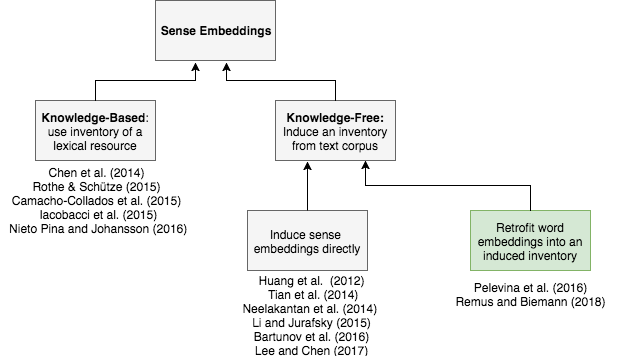
\includegraphics[height=0.56\textwidth]{GWC-1}
 \end{center}
\end{frame}


\begin{frame}
\frametitle{Related work: knowledge-based}
\begin{itemize}
	\item \textbf{AutoExtend}~\cite{rothe-schutze:2015:ACL-IJCNLP}
\end{itemize}
\begin{center}
 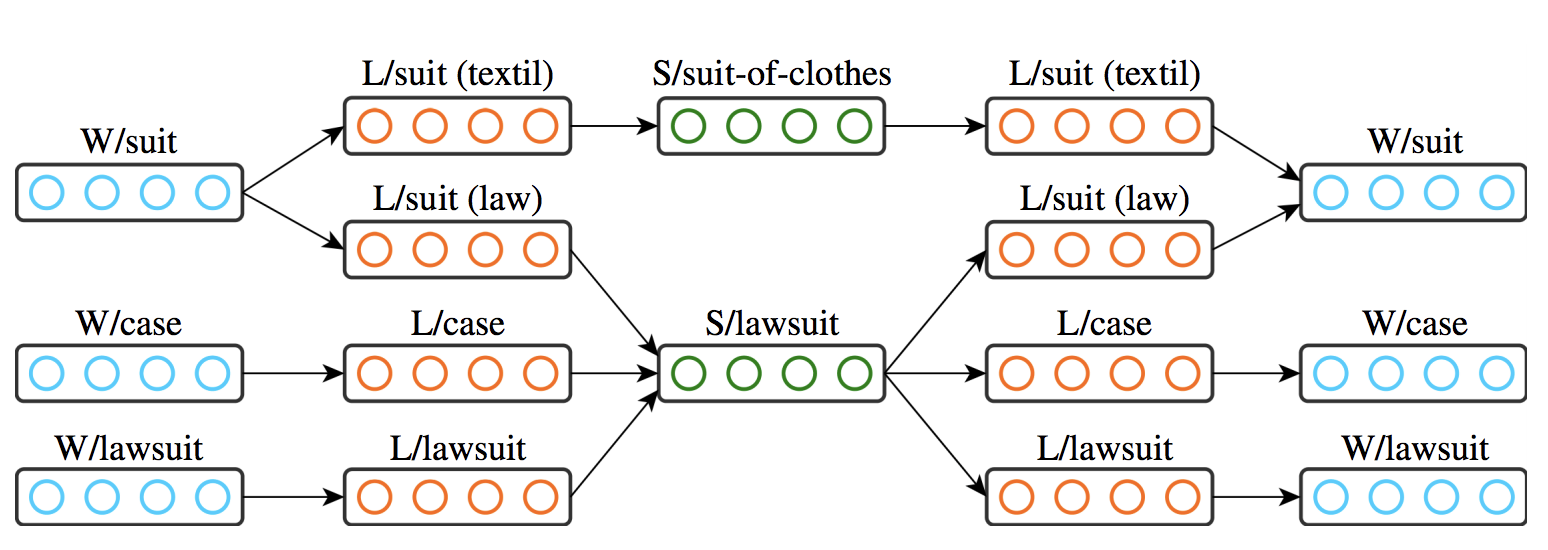
\includegraphics[width=1.0\textwidth]{autoextend}
 \end{center}

{\footnotesize
 * image is reproduced from the original paper
}

\end{frame}

\begin{frame}{Related work: knowledge-free}

\begin{itemize}
\item \textbf{Adagram}~\cite{bartunov2016breaking}
\item Multiple vector representations $\theta$ for each word:

\pause
 $$p(Y,\textcolor{Cerulean}{Z},\mathbf{\beta}|X,\alert{\alpha},\theta) = \prod_{w=1}^{V} \prod_{k=1}^{\infty} p(\beta_{wk}|\alert{\alpha}) \prod_{i=1}^N [p(\textcolor{Cerulean}{z_i}|x_i,\mathbf{\beta}) \prod_{j=1}^C p(y_{ij}|\textcolor{Cerulean}{z_i},x_i,\theta)],$$ 
\begin{itemize}
 
\item $\textcolor{Cerulean}{z_i}$ -- a hidden variable: a sense index of word $x_i$ in context $C$; 
\item $\alert{\alpha}$ -- a meta-parameter controlling number of senses.
%\item $p(\beta_{wk}|\alpha)$ -- probability of the $k$-th sense of the word $w$;
%\item $p(z_i|x_i,\mathbf{\beta})$ -- probability of observing word $x_i$ in the sense $z_i$;
%\item $\prod_{j=1}^C p(y_{ij}|z_i,x_i,\theta)$ -- probability of the context $C$.
\end{itemize}

\pause 
\item \alert{\textbf{See also}}: [Neelakantan et al., 2014] and [Li and Jurafsky, 2015]

\end{itemize}
	
\end{frame}


\begin{frame}{Related work: word sense induction}

\begin{itemize}
	\item Word sense induction (WSI) based on \alert{\textbf{graph clustering}}:  
	\begin{itemize}
	\item $ $ [Lin, 1998]
	\item $ $ [Pantel and Lin, 2002]
	\item $ $ [Widdows and Dorow, 2002]
	\item $ $ \textbf{Chinese Whispers [Biemann, 2006]}
	\item $ $ [Hope and Keller, 2013]
	\end{itemize}
	
	%\item ...we extend this line of work.
\end{itemize}
	

\end{frame}



\begin{frame}[fragile]
\frametitle{Related work: Chinese Whispers\#1}
\begin{center}
 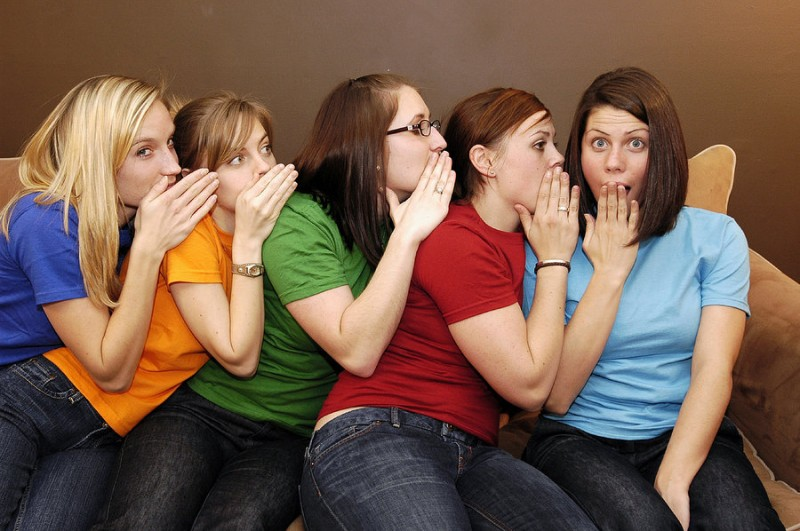
\includegraphics[height=0.5\textwidth]{cw}
 
  {\tiny * source of the image: \url{http://ic.pics.livejournal.com/blagin_anton/33716210/2701748/2701748_800.jpg}}
 \end{center}
\end{frame}



\begin{frame}[fragile]
\frametitle{Related work: Chinese Whispers\#2}
\begin{center}
 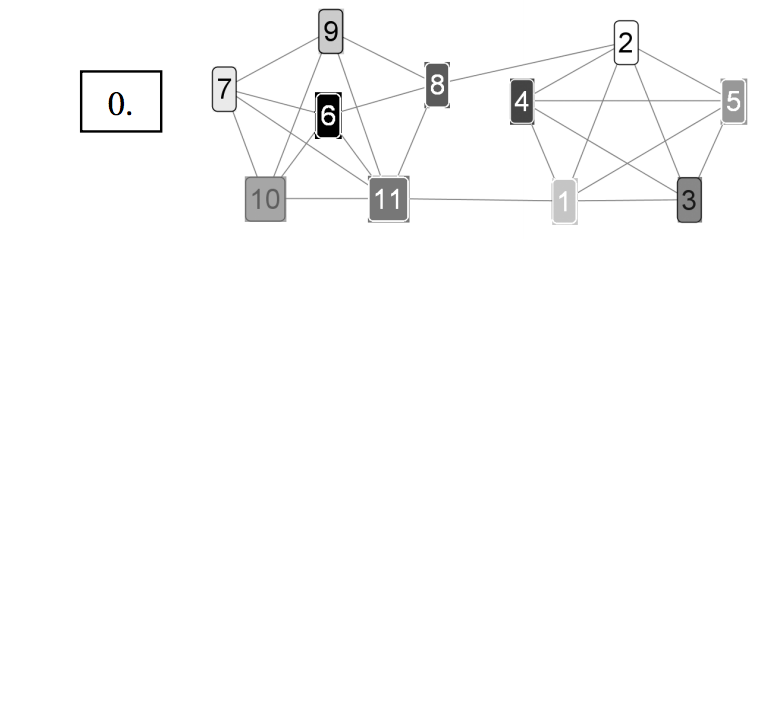
\includegraphics[height=0.59\textwidth]{cw2-1}
 
  %{\tiny * source of the image: [Biemann, 2006]}
 \end{center}
\end{frame}


\begin{frame}[fragile]
\frametitle{Related work: Chinese Whispers\#2}
\begin{center}
 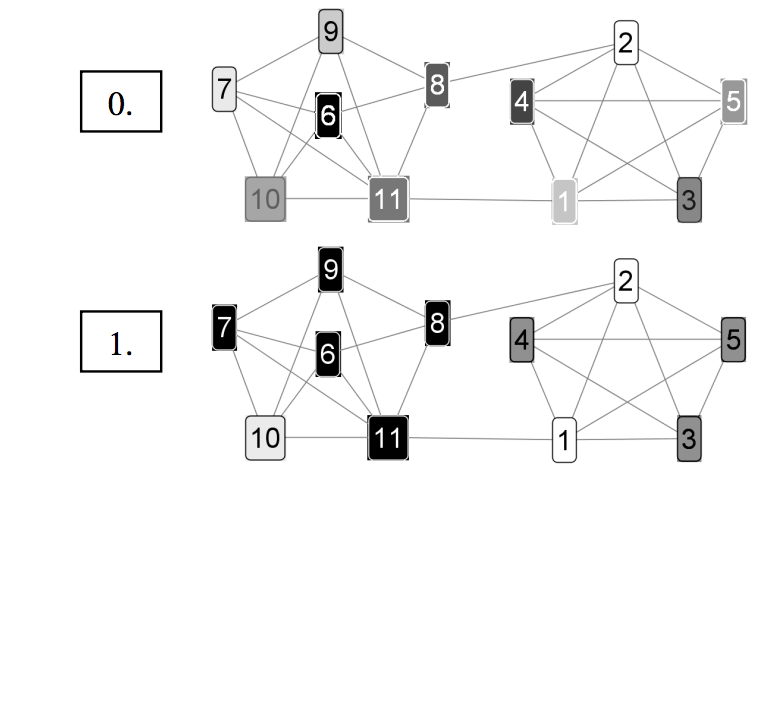
\includegraphics[height=0.59\textwidth]{cw2-2}
 
  %{\tiny * source of the image: [Biemann, 2006]}
 \end{center}
\end{frame}

\begin{frame}[fragile]
\frametitle{Related work: Chinese Whispers\#2}
\begin{center}
 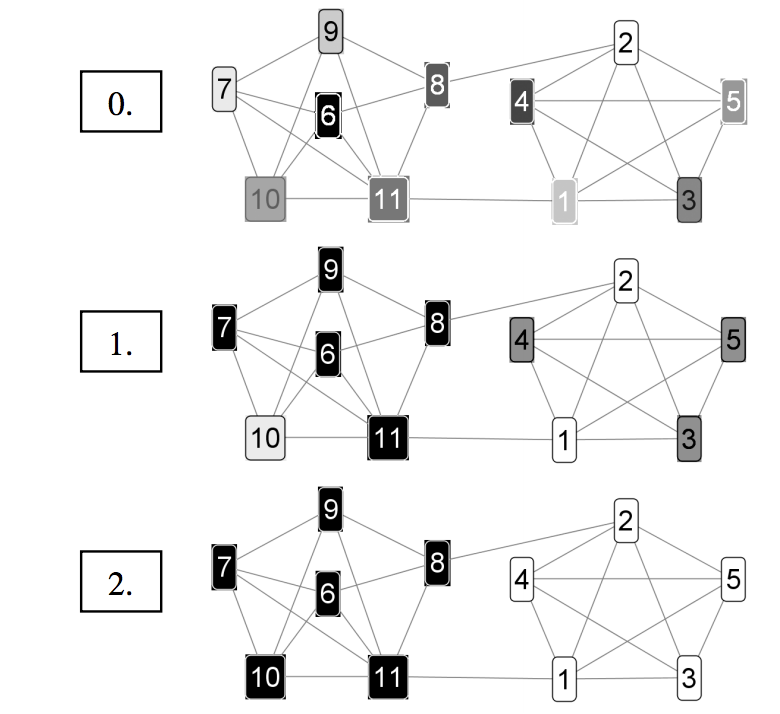
\includegraphics[height=0.59\textwidth]{cw2}
 
  %{\tiny * source of the image: [Biemann, 2006]}
 \end{center}
\end{frame}



\begin{frame}{Sense embeddings using retrofitting}
	
	%\begin{itemize} 
	 {\footnotesize \textbf{RepL4NLP@ACL'16} \cite{pelevina-EtAl:2016:RepL4NLP}, \textbf{LREC'18} \cite{remus:2018}}
	%\end{itemize}
	
	\begin{block}{Prior methods:}
		\vspace{0.25cm}

	\begin{itemize}	
	\item Induce inventory by \alert{clustering of word instances} %(Li and Jurafsky, 2015)
	\item Use \alert{existing} sense inventories %(Rothe and Sch\"{u}tze, 2015)	
	\end{itemize}
\end{block}


	\begin{block}{Our method:}
		\vspace{0.25cm}

	\begin{itemize}	
	\item \textbf{Input:} word embeddings
	\item \textbf{Output:} word sense embeddings
	\item \textbf{Word sense induction} by \alert{clustering of word ego-networks}
	%\item \textbf{Word sense disambiguation} based on the induced sense representations

	\end{itemize}
\end{block}


\end{frame}

\begin{frame}{Sense embeddings using retrofitting}
\begin{itemize}
\item From word embeddings to sense embeddings
\end{itemize}
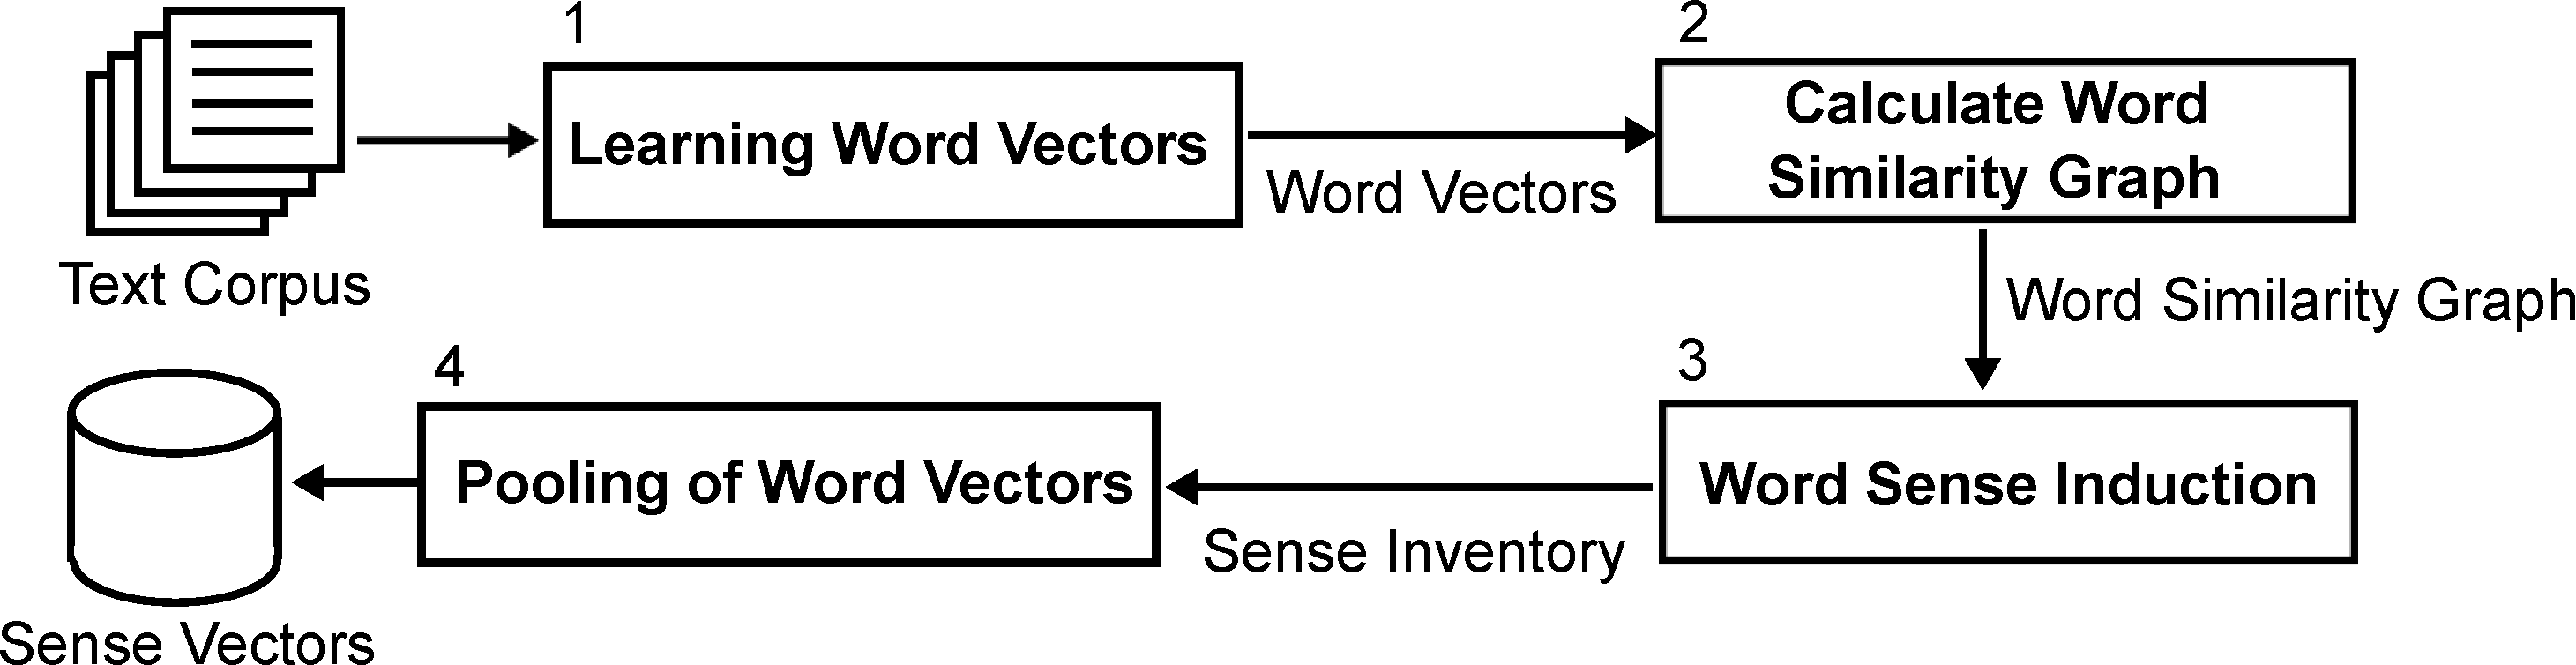
\includegraphics[width=\textwidth]{pipeline-sensegram}
%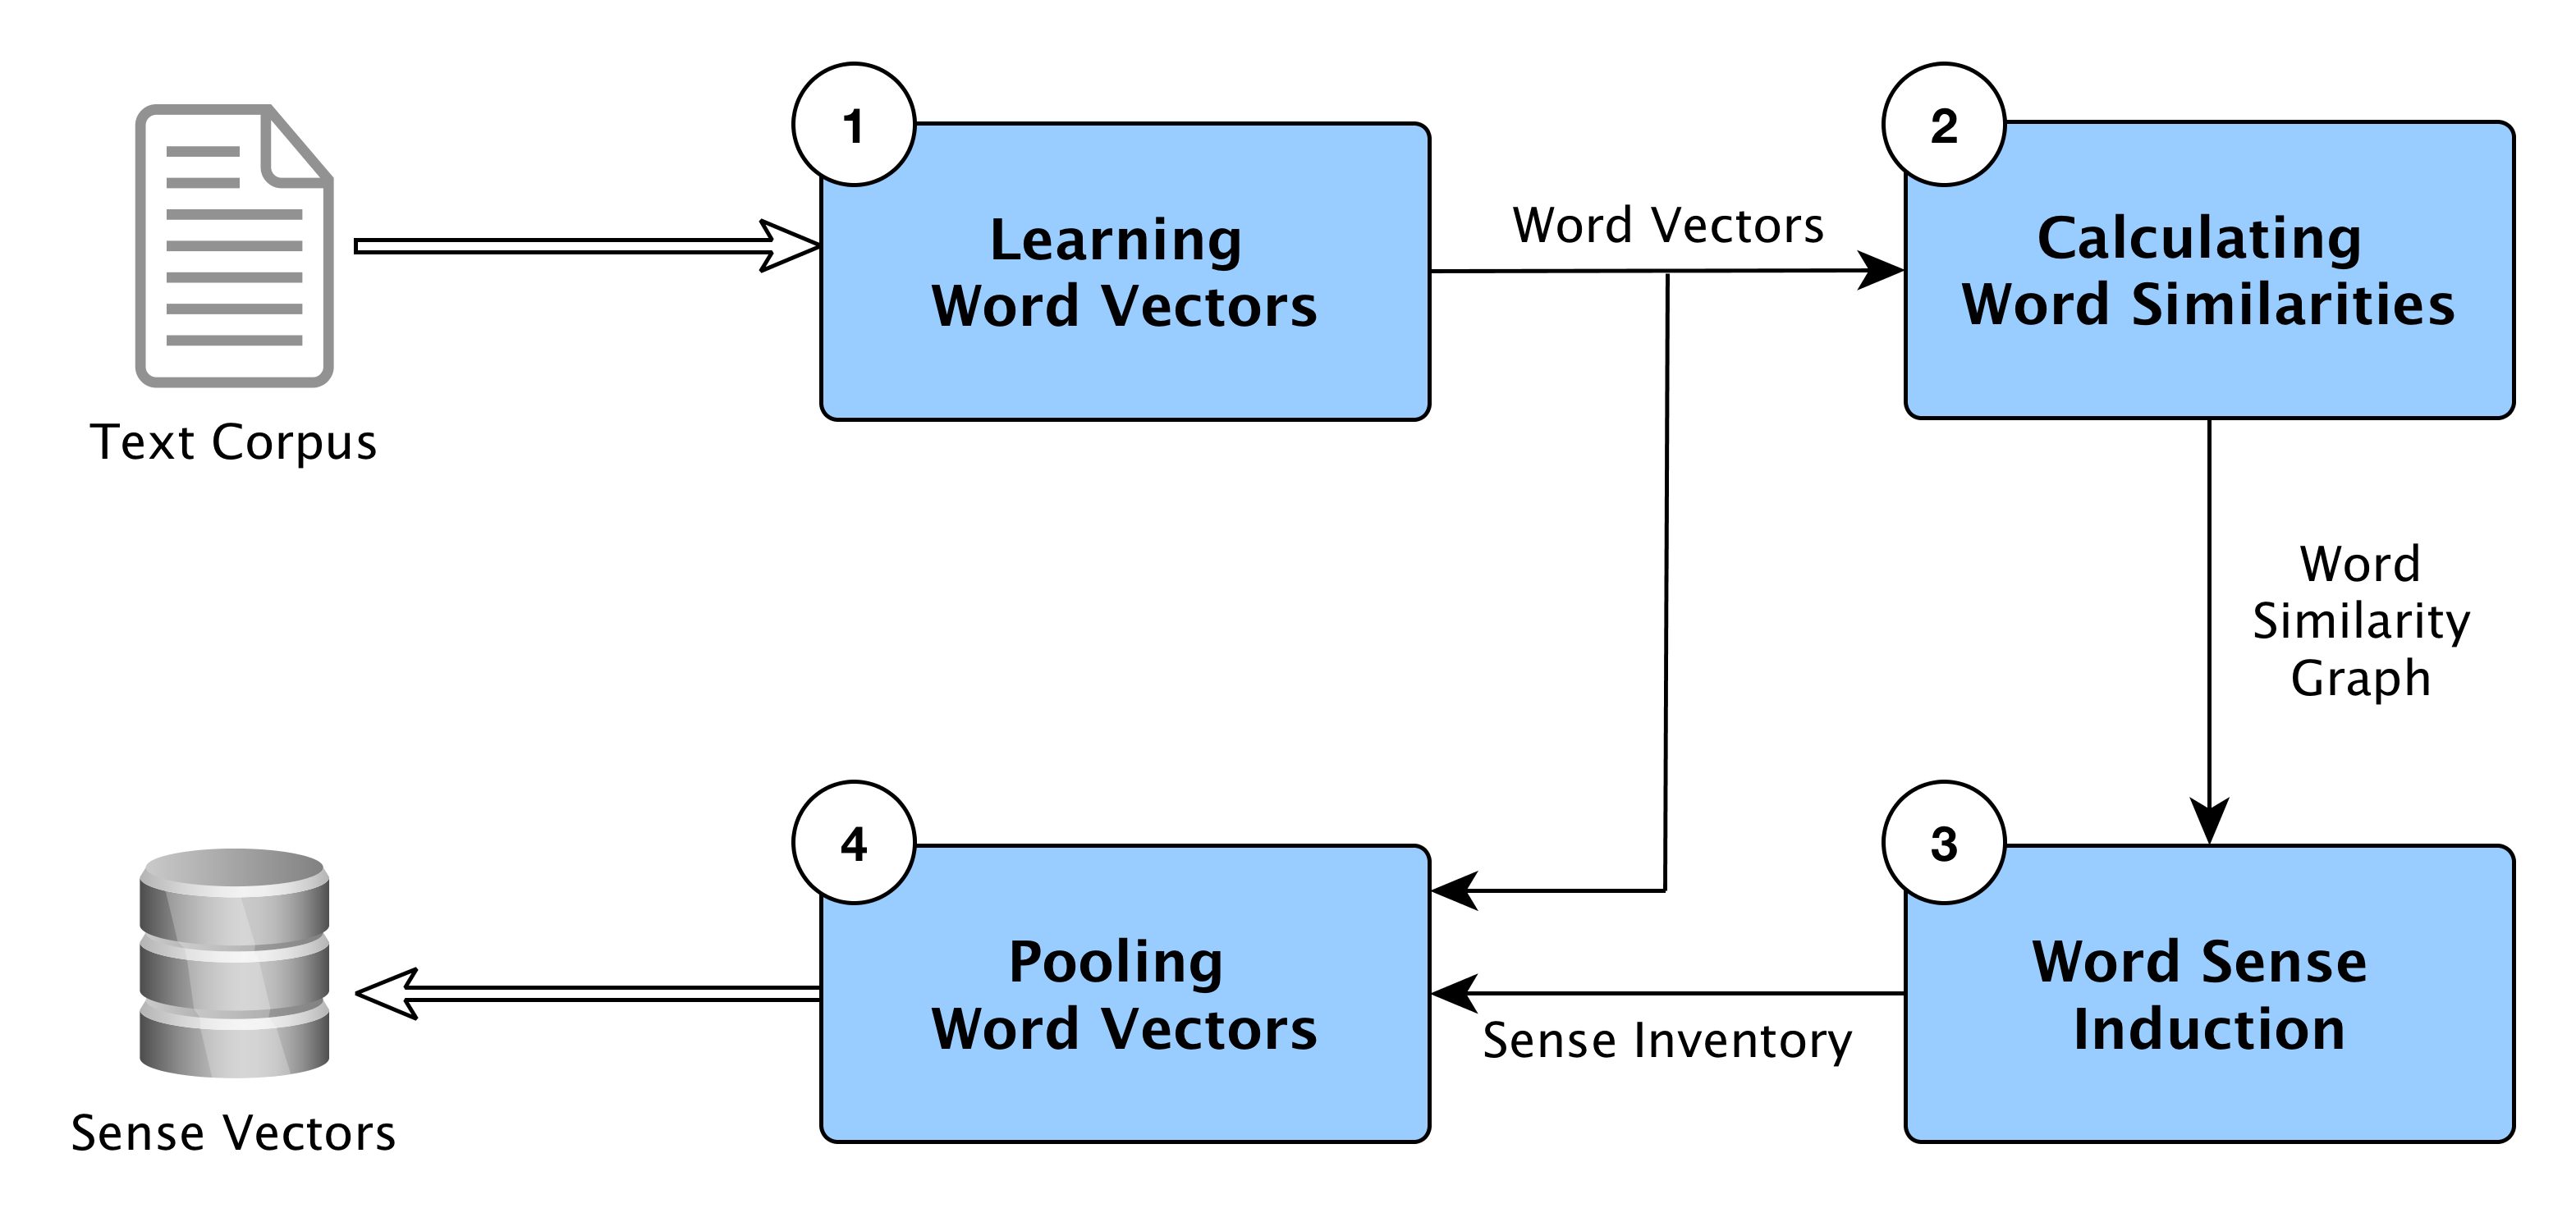
\includegraphics[width=\textwidth]{pipeline}

\end{frame}



\begin{frame}{Sense embeddings using retrofitting}

\begin{itemize}
\item Word sense induction using  ego-network clustering
\end{itemize} 
	
\centering
\begin{figure}
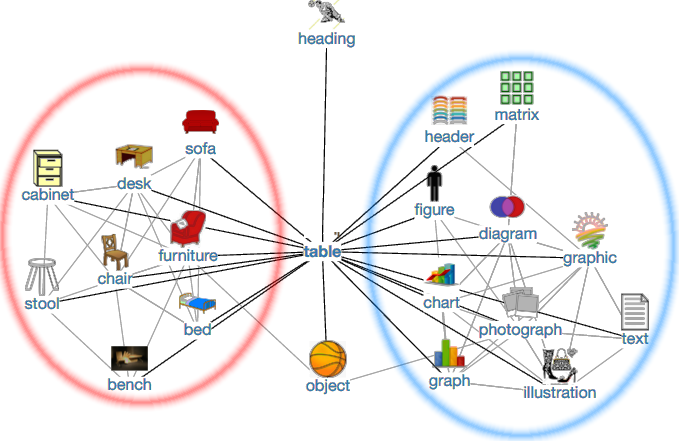
\includegraphics[width=0.75\textwidth]{table}
\end{figure}

\end{frame}


\begin{frame}{Sense embeddings using retrofitting}

\begin{itemize}
	\item Neighbours of Word and Sense Vectors
\end{itemize}


%\begin{table}
%
%\footnotesize
%\centering

\begin{tabular}{l|p{9cm}}
\bf Vector & \bf {Nearest Neighbors} \\ \toprule
 table & $ $ \alert{tray}, \textcolor{Cerulean}{bottom}, \textcolor{Cerulean}{diagram}, \alert{bucket}, \textcolor{Cerulean}{brackets}, \textcolor{Cerulean}{stack}, \alert{basket}, \textcolor{Cerulean}{list}, \textcolor{Cerulean}{parenthesis}, \alert{cup}, \alert{saucer}, \alert{pile}, \alert{playfield}, \textcolor{Cerulean}{bracket}, \alert{pot}, \textcolor{Cerulean}{drop-down}, \alert{cue}, \alert{plate} \\ \midrule
 \pause
  \textcolor{Cerulean}{table\#0} & $ $ \textcolor{Cerulean}{leftmost\#0},  \textcolor{Cerulean}{column\#1},  \textcolor{Cerulean}{tableau\#1},  \textcolor{Cerulean}{indent\#1},  \textcolor{Cerulean}{bracket\#3},  \textcolor{Cerulean}{pointer\#0},  \textcolor{Cerulean}{footer\#1}, \textcolor{Cerulean}{cursor\#1}, \textcolor{Cerulean}{diagram\#0}, \textcolor{Cerulean}{grid\#0} \\ \midrule
   \alert{table\#1} & $ $ \alert{pile\#1,  stool\#1,  tray\#0,  basket\#0,  bowl\#1,  bucket\#0,  box\#0,  cage\#0,  saucer\#3,      mirror\#1,  pan\#1,  lid\#0}  \\ 
\end{tabular}
	

\end{frame}




\begin{frame}{Sense embeddings using retrofitting}
	
	\begin{block}{Word Sense Disambiguation}
	
	\begin{enumerate} 
	\item \textbf{\alert{Context extraction}}: use context words around the target word
	\item \textbf{\alert{Context filtering}}: based on context word's relevance for disambiguation
	
	\item \textbf{\alert{Sense choice in context}}: maximise similarity between a context vector and a sense vector
	
	\end{enumerate}
	\end{block}

\end{frame}


\begin{frame}{Sense embeddings using retrofitting}
\vspace{-3em}
\begin{center}
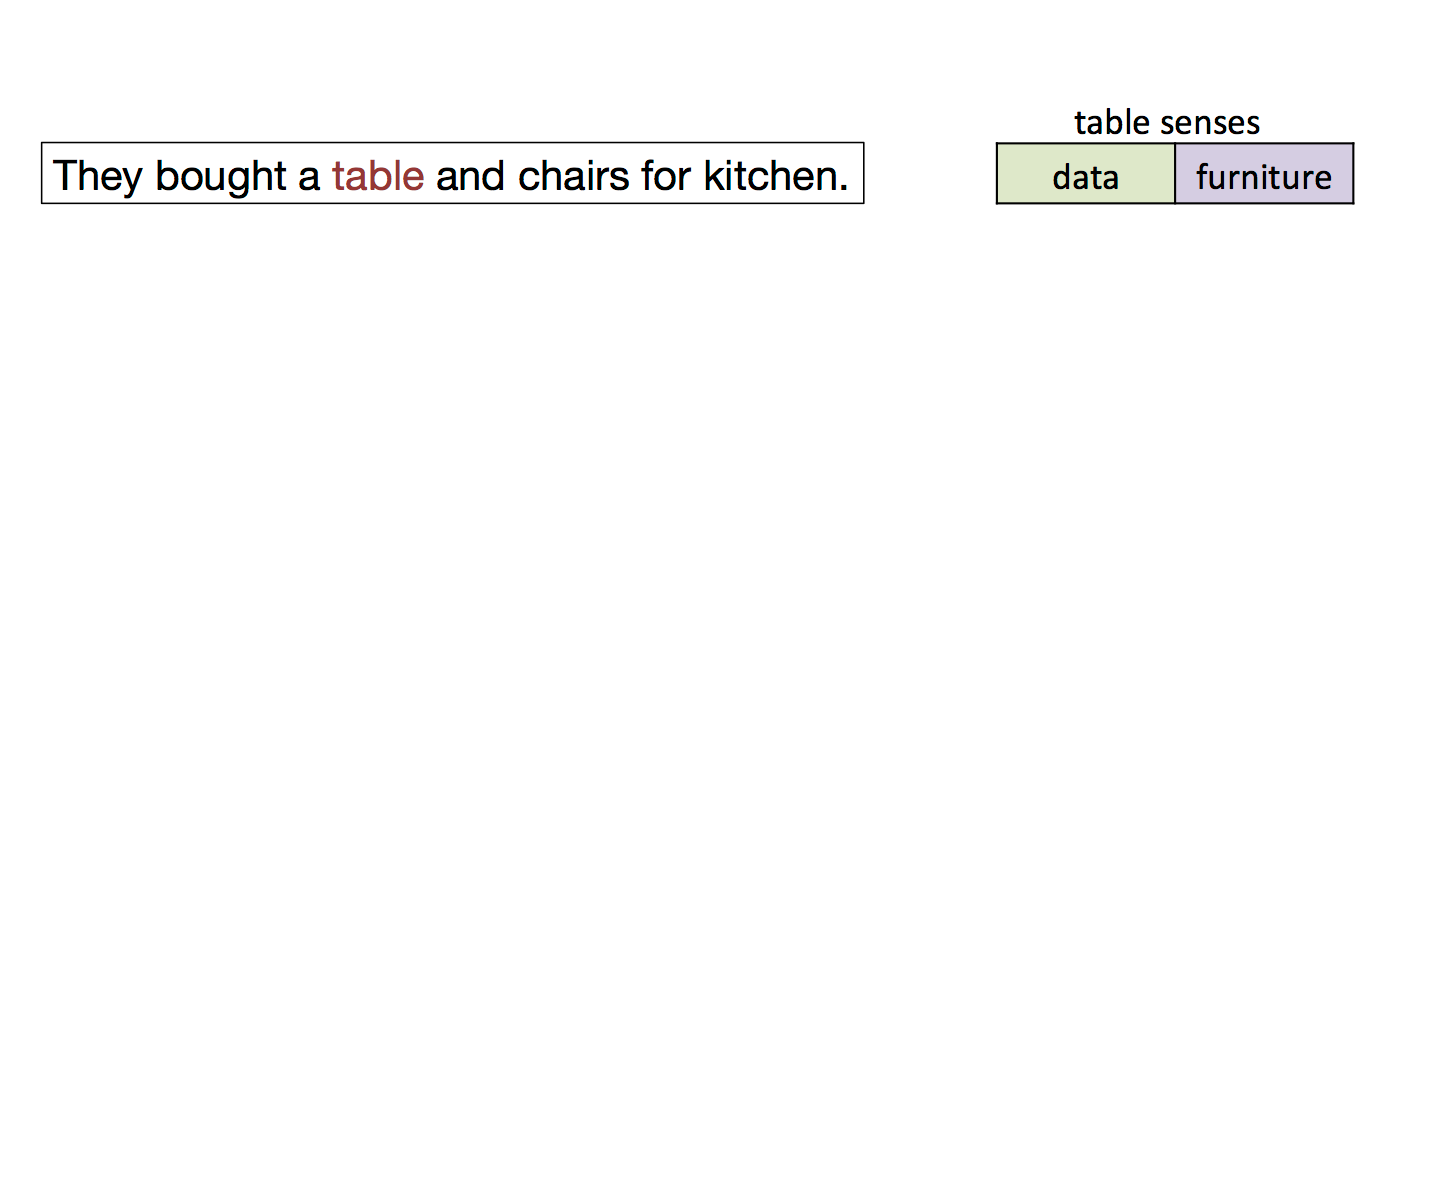
\includegraphics[width=0.82\textwidth]{wsd-1}
\end{center}	
\end{frame}



\begin{frame}{Sense embeddings using retrofitting}
\vspace{-3em}
\begin{center}
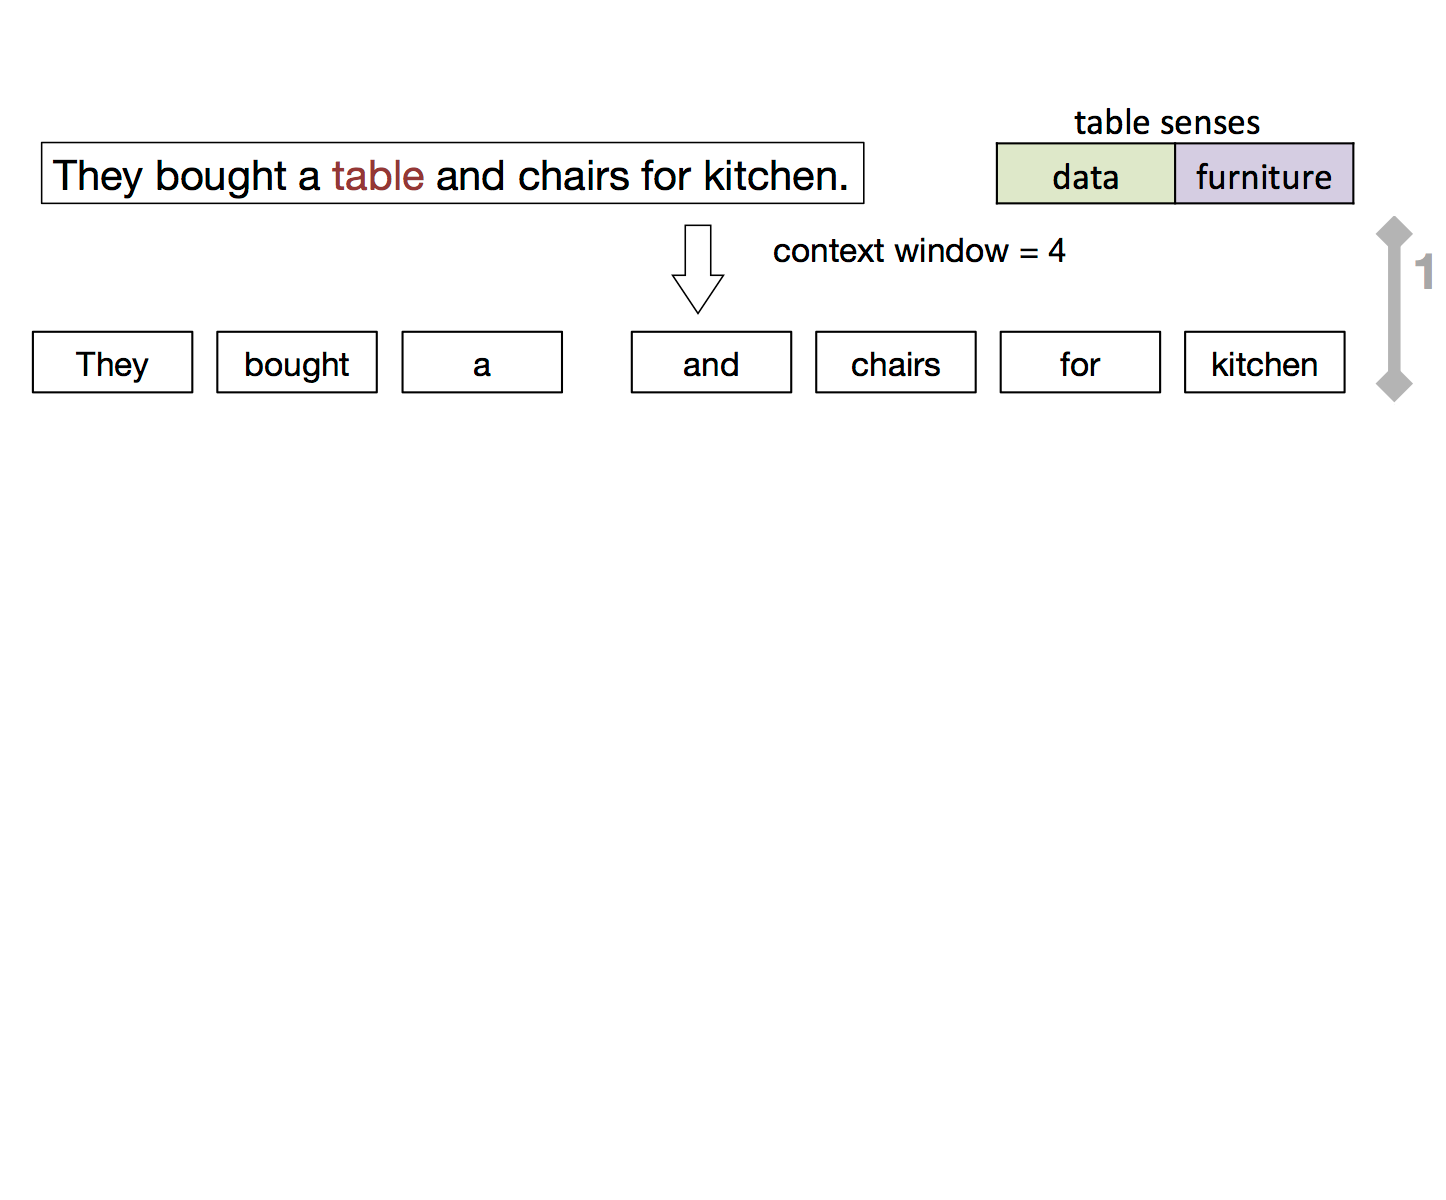
\includegraphics[width=0.82\textwidth]{wsd-2}
\end{center}	
\end{frame}



\begin{frame}{Sense embeddings using retrofitting}
\vspace{-3em}
\begin{center}
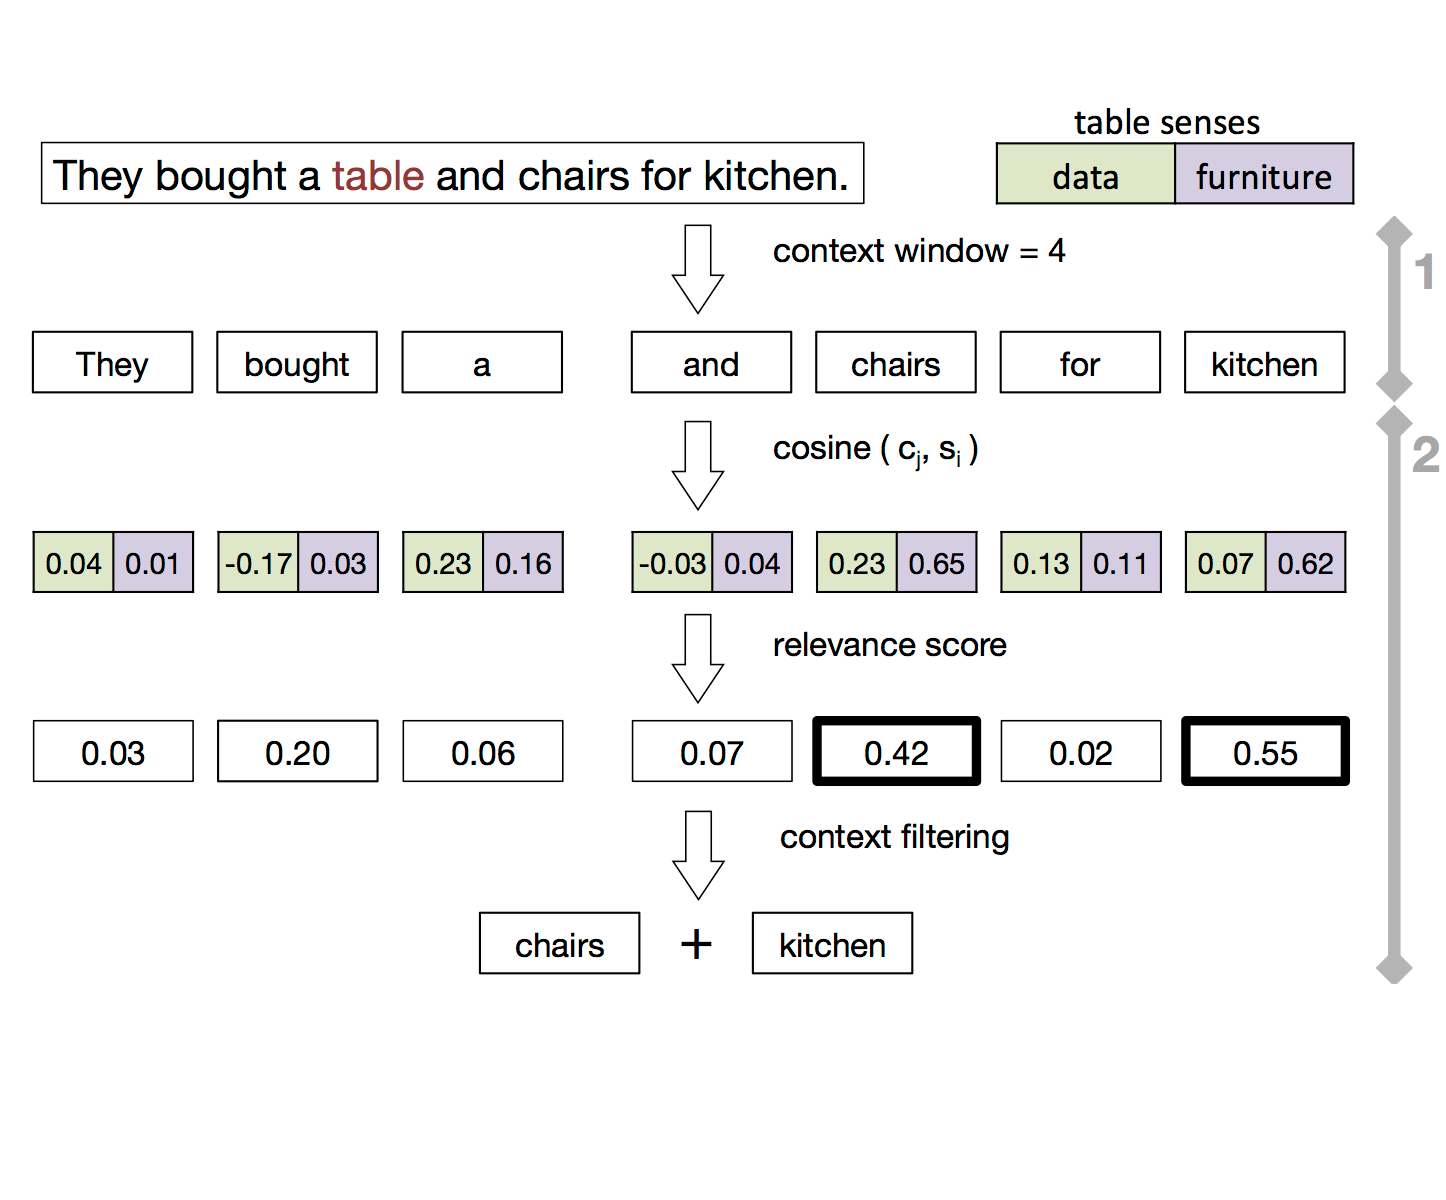
\includegraphics[width=0.82\textwidth]{wsd-3}
\end{center}	
\end{frame}



	
\begin{frame}{Sense embeddings using retrofitting}
%\begin{itemize}
%	\item An example of word sense disambiguation
%\end{itemize}
\vspace{-3em}
	\begin{center}
		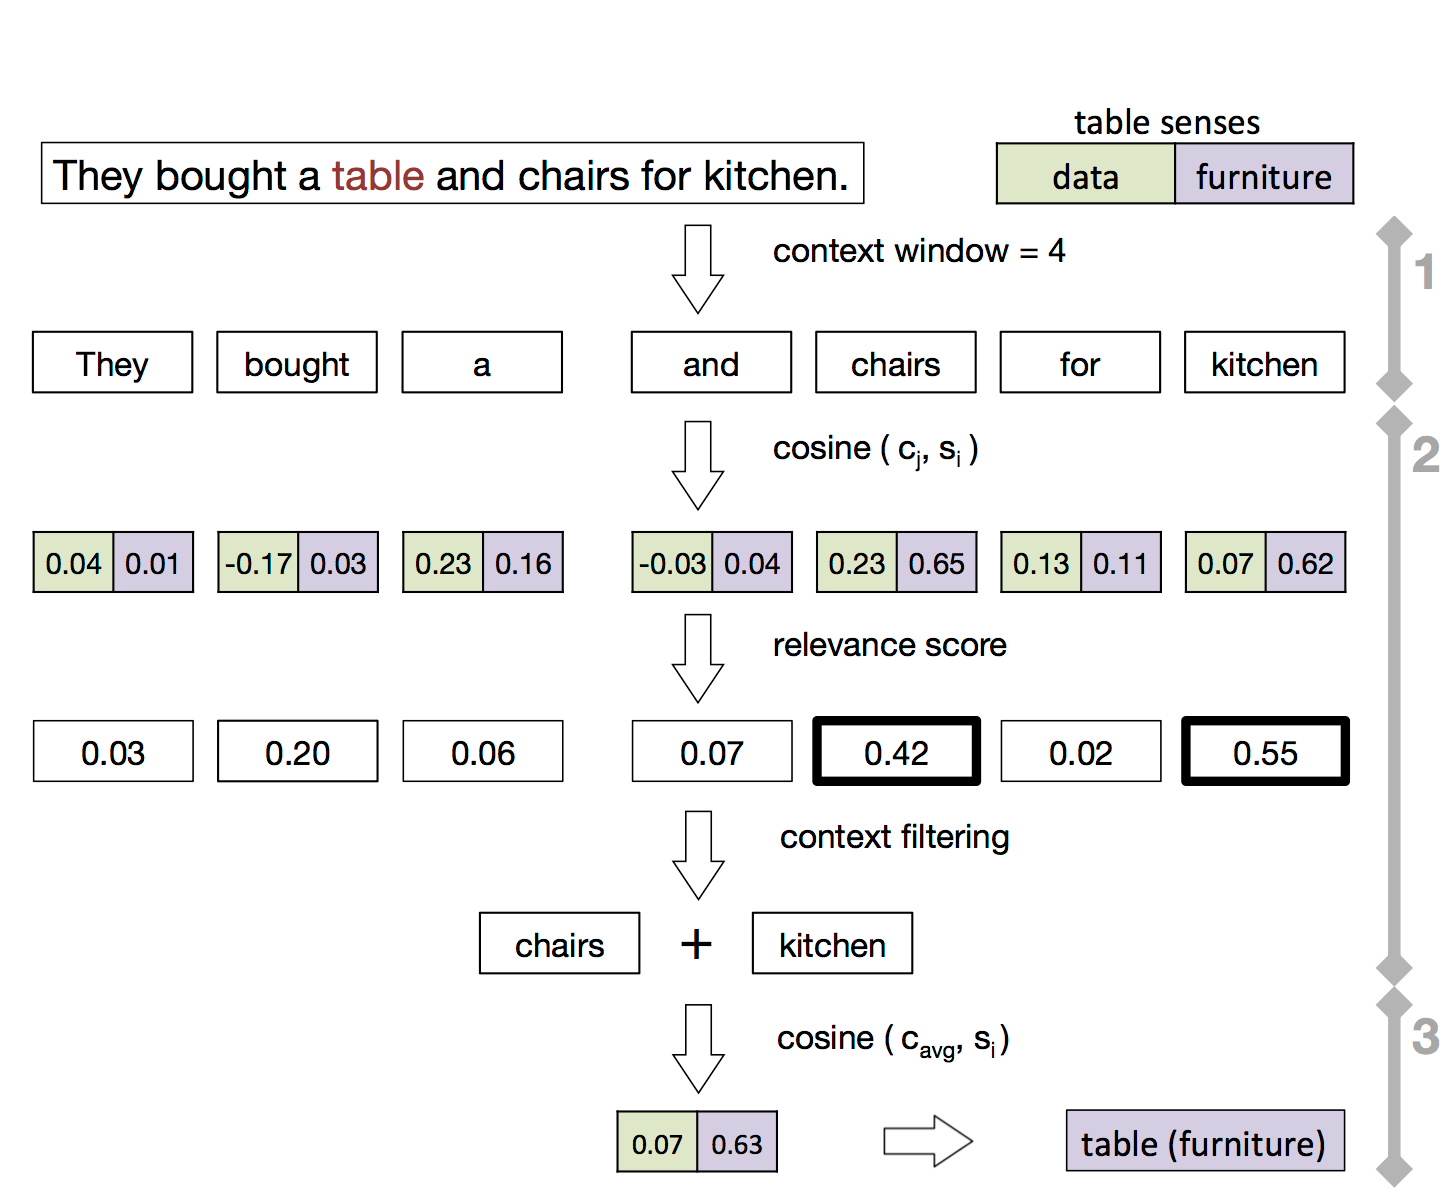
\includegraphics[width=0.82\textwidth]{wsd}
	\end{center}
	
\end{frame}






\begin{frame}{Sense embeddings using retrofitting}

\alert{\textbf{Unsupervised WSD}} SemEval'13, \textbf{ReprL4NLP}~\cite{pelevina-EtAl:2016:RepL4NLP}:
\begin{itemize}
	\item comparable to SOTA, incl. sense embeddings.
\end{itemize} 

\vspace{2em}
\alert{\textbf{Semantic relatedness}}, \textbf{LREC'2018}~\cite{remus:2018}:
\vspace{2em}
\begin{table}
    \tiny
 	
 	\def\arraystretch{1.2}% 
 	\setlength{\arraycolsep}{3pt}
 	
 	$$
 	\begin{array}{rll|ll|ll|ll|ll|ll|ll}
 	  & \rotatebox{80}{\textsc{autoextend}\hspace{-10em}} 
 	  & \rotatebox{80}{\textsc{adagram}\hspace{-10em}} 
 	  & ~\rotatebox{80}{\textsc{SGNS}\hspace{-10em}} 
 	  & \rotatebox{80}{\textsc{.}\hspace{-10em}} 
 	  & \rotatebox{80}{\textsc{glove}\hspace{-10em}} 
 	  & \rotatebox{80}{\textsc{.}\hspace{-10em}} 
 	  & \rotatebox{80}{\textsc{sympat}\hspace{-10em}} 
 	  & \rotatebox{80}{\textsc{.}\hspace{-10em}} 
 	  & \rotatebox{80}{\textsc{LSAbow}\hspace{-10em}} 
 	  & \rotatebox{80}{\textsc{.}\hspace{-10em}}
 	  & \rotatebox{80}{\textsc{LSAhal}\hspace{-10em}}
	  & \rotatebox{80}{\textsc{.}\hspace{-10em}}
	  & ~~\rotatebox{80}{\textsc{paragramSL}\hspace{-10em}} 
 	  & \rotatebox{80}{\textsc{.}\hspace{-10em}}  
 	  \\
   	 \textsc{SimLex999}  & 0.45 & 0.29 ~~&~ 0.44 &  & 0.37 &  & 0.54 &  & 0.30 &  & 0.27 & & ~ {0.68} &  \\
   	 \textsc{MEN} & 0.72 & 0.67 &~   0.77 &  & 0.73 &  & 0.53 &  & 0.67 &  & 0.71 &  &~ 0.77 &  \\
   	 \textsc{SimVerb} & 0.43 & 0.27 &~   0.36 &  & 0.23 &  & 0.37 &  & 0.15 &  & 0.19 &  &~ 0.53 &  \\
   	 \textsc{WordSim353} & 0.58 & 0.61 &~   {0.70} &  & 0.61 &  & 0.47 & & {0.67} &  & 0.59 & &~ 0.72 & \\ 

   	 \textsc{SimLex999-N}  & 0.44 & 0.33 ~~&~ 0.45 &  & 0.39 &  & 0.48 &  & 0.32 & & 0.34 & & {0.68} & \\
   	 \textsc{MEN-N} 		 & 0.72 & 0.68 &~   0.77 & \_\_\_\_ & 0.76 & \_\_\_\_ & 0.57 & \_\_\_\_ & 0.71 & \_\_\_\_ & 0.73 & \_\_\_\_ &~ 0.78 & \_\_\_\_ \\
 	\end{array}
 	$$
 
 \end{table}


\end{frame}



\begin{frame}{Sense embeddings using retrofitting}

\alert{\textbf{Unsupervised WSD}} SemEval'13, \textbf{ReprL4NLP}~\cite{pelevina-EtAl:2016:RepL4NLP}:
\begin{itemize}
	\item comparable to SOTA, incl. sense embeddings.
\end{itemize} 

\pause

\vspace{2em}

\alert{\textbf{Semantic relatedness}}, \textbf{LREC'2018}~\cite{remus:2018}:
\vspace{2em}
\begin{table}
    \tiny
 	
 	\def\arraystretch{1.2}% 
 	\setlength{\arraycolsep}{3pt}
 	
 	$$
 	\begin{array}{rll|ll|ll|ll|ll|ll|ll}
 	  & \rotatebox{80}{\textsc{autoextend}\hspace{-10em}} 
 	  & \rotatebox{80}{\textsc{adagram}\hspace{-10em}} 
 	  & ~\rotatebox{80}{\textsc{SGNS}\hspace{-10em}} 
 	  & \rotatebox{80}{\textsc{SGNS\alert{+senses}}\hspace{-10em}} 
 	  & \rotatebox{80}{\textsc{glove}\hspace{-10em}} 
 	  & \rotatebox{80}{\textsc{glove\alert{+senses}}\hspace{-10em}} 
 	  & \rotatebox{80}{\textsc{sympat}\hspace{-10em}} 
 	  & \rotatebox{80}{\textsc{sympat\alert{+senses}}\hspace{-10em}} 
 	  & \rotatebox{80}{\textsc{LSAbow}\hspace{-10em}} 
 	  & \rotatebox{80}{\textsc{LSAbow\alert{+senses}}\hspace{-10em}}
 	  & \rotatebox{80}{\textsc{LSAhal}\hspace{-10em}}
	  & \rotatebox{80}{\textsc{LSAhal\alert{+senses}}\hspace{-10em}}
	  & ~~\rotatebox{80}{\textsc{paragramSL}\hspace{-10em}} 
 	  & \rotatebox{80}{\textsc{paragramSL\alert{+senses}}\hspace{-10em}}  
 	  \\
   	 \textsc{SimLex999}  & 0.45 & 0.29 ~~&~ 0.44 & \mathbf{0.46} & 0.37 & \bf0.41 & 0.54 & \mathbf{0.55} & 0.30 & \bf0.39 & 0.27 & \bf0.38 ~& \mathbf{0.68} & {0.64} \\
   	 \textsc{MEN} 		 & 0.72 & 0.67 &~   0.77 & \mathbf{0.78} & 0.73 & \bf0.77 & 0.53 & \bf0.68 & 0.67 & \bf0.70 & 0.71 & \bf0.74 &~ 0.77 & \bf0.80  \\
   	 \textsc{SimVerb} 	 & 0.43 & 0.27 &~   0.36 & \bf0.39 & 0.23 & \bf0.30 & 0.37 & \bf0.45 & 0.15 & \bf0.22 & 0.19 & \bf0.28 & 0.53 & 0.53 \\
   	 \textsc{WordSim353} & 0.58 & 0.61 &~   \mathbf{0.70} & 0.69 & 0.61 & \bf0.65 & 0.47 & \bf0.62 & \mathbf{0.67} & 0.66 & 0.59 & \bf0.63 &~ 0.72 & \mathbf{0.73} \\ 

   	 \textsc{SimLex999-N}  & 0.44 & 0.33 ~~&~ 0.45 & \bf0.50 & 0.39 & \bf0.47 & 0.48 & \bf0.55 & 0.32 & \bf0.46 & 0.34 & \bf 0.44 & \mathbf{0.68} & {0.66} \\
   	 \textsc{MEN-N} 		 & 0.72 & 0.68 &~   0.77 & \mathbf{0.79} & 0.76 & \bf0.80 & 0.57 & \bf0.74 & 0.71 & \mathbf{0.73} & 0.73 & \bf0.76 &~ 0.78 & \bf 0.81 \\
 	\end{array}
 	$$
 
 \end{table}
%\vspace{-1em}
%\begin{itemize}
%
%\item Sense-aware similarities are marked with \alert{\textsc{+SENSES}}.
%\item These results are using a sense inventory based on \textbf{sparse dependency features} (JoBimText).
%
%\end{itemize}

\end{frame}



\begin{frame}{Sense embeddings using retrofitting}
\vspace{-1em}
\begin{columns}
\begin{column}{0.55\textwidth}
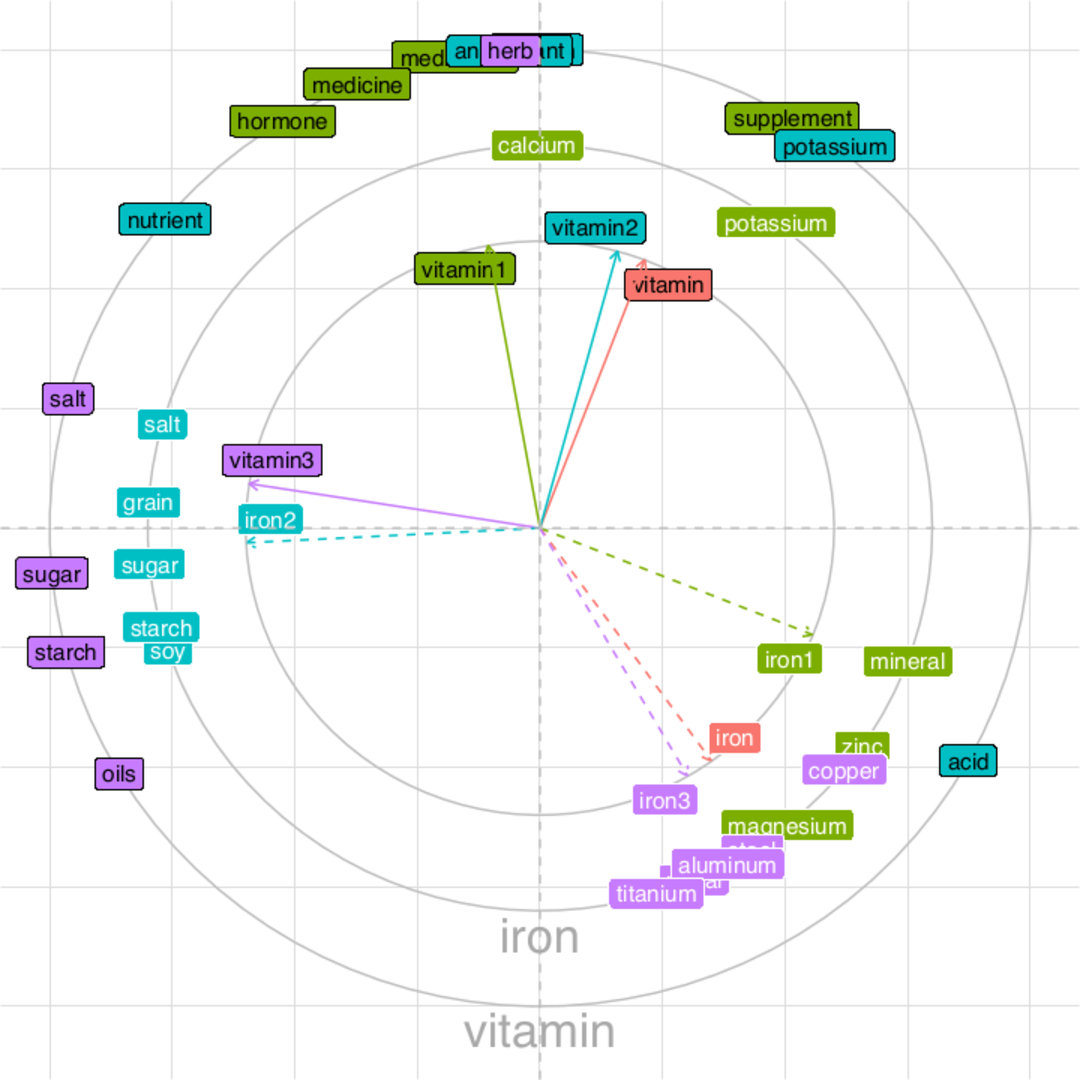
\includegraphics[height=0.68\textheight]{bullseye}
\end{column}

\begin{column}{.45\textwidth}
{ \footnotesize

\begin{itemize}

\item Word and sense embeddings of words \textbf{iron} and  \textbf{vitamin}.

\end{itemize}

\textbf{LREC'18}~\cite{remus:2018}

}
\end{column}
\end{columns}

\end{frame}

%%%%%%%%%%%%%%%%%%%%%%%%% 


%
%\begin{frame}{Synset induction}
%	\textbf{ACL'17}~\cite{ustalov-panchenko-biemann:2017:Long}
%	
%	
%	%\block{Sample Synsets Induced by the \watset{[MCL, MCL]} Method for English}{
%\vspace{1em}
%Examples of extracted synsets:
%\vspace{1em}
%\centering
%\begin{tabular}{c|p{9cm}}
%\textbf{Size} & \textbf{Synset}\\\hline
%2 & \{\textit{decimal point}, \textit{dot}\}\\
%3 & \{\textit{gullet}, \textit{throat}, \textit{food pipe}\}\\
%4 & \{\textit{microwave meal}, \textit{ready meal}, \textit{TV dinner}, \textit{frozen dinner}\}\\
%5 & \{\textit{objective case}, \textit{accusative case}, \textit{oblique case}, \textit{object case}, \textit{accusative}\}\\
%6 & \{\textit{radio theater}, \textit{dramatized audiobook}, \textit{audio theater}, \textit{radio play}, \textit{radio drama}, \textit{audio play}\}\\
%\end{tabular}
%
%
%	
%	
%\end{frame}
%
%
%\begin{frame}{Synset induction}
%	
%	
%Outline of the 'Watset' method:
%
%\vspace{2em}
%
%\centering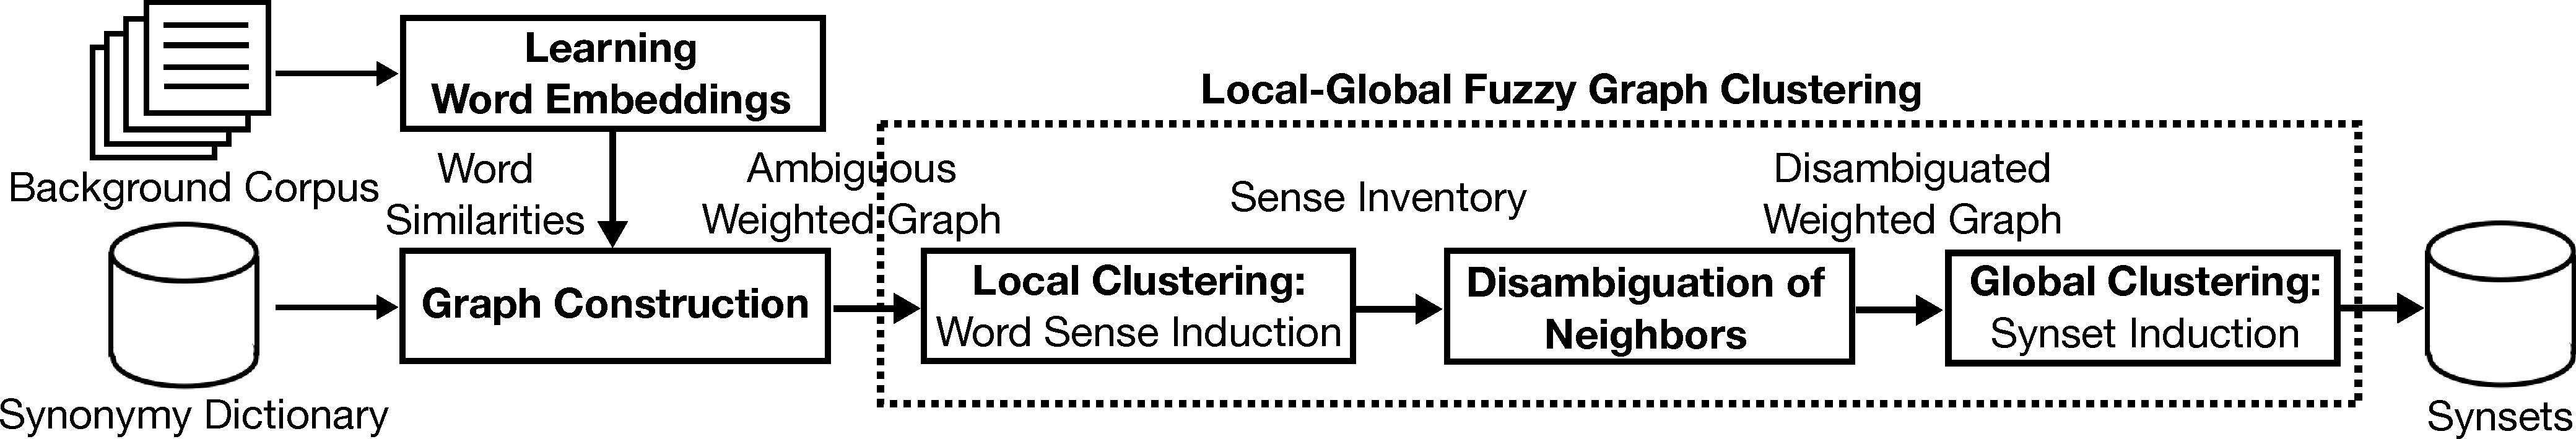
\includegraphics[width=1.05\textwidth]{figures/outline}
%	
%\end{frame}
%
%
%\begin{frame}{Synset induction}
%\centering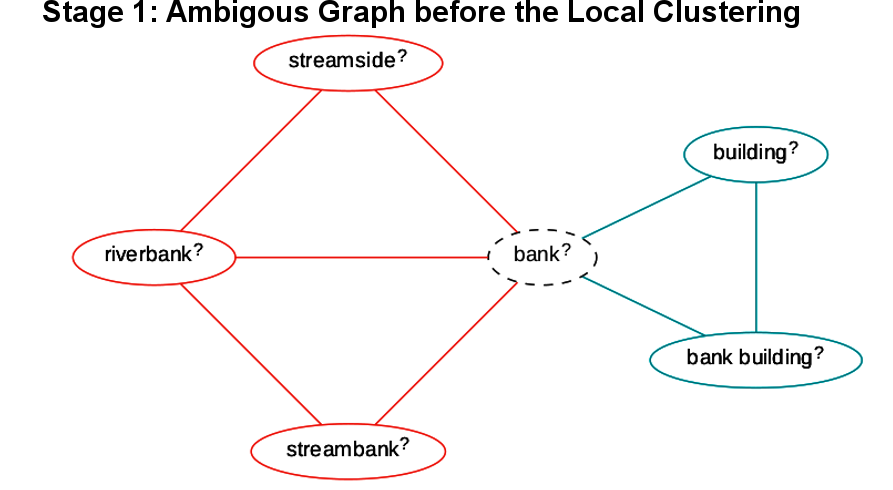
\includegraphics[width=1\textwidth]{figures/stages1}	
%\end{frame}
%
%
%
%\begin{frame}{Synset induction}
%\centering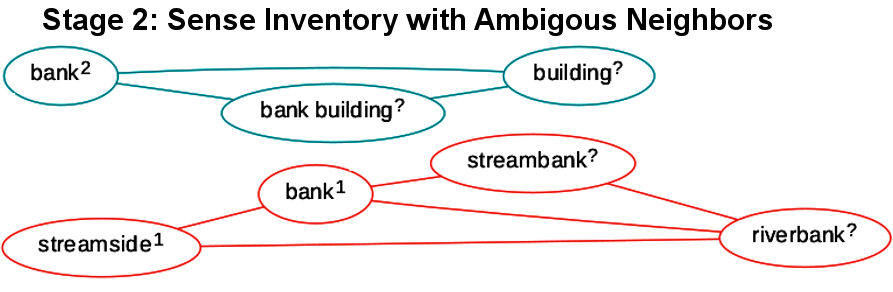
\includegraphics[width=1\textwidth]{figures/stages2}	
%\end{frame}
%
%
%
%\begin{frame}{Synset induction}
%\centering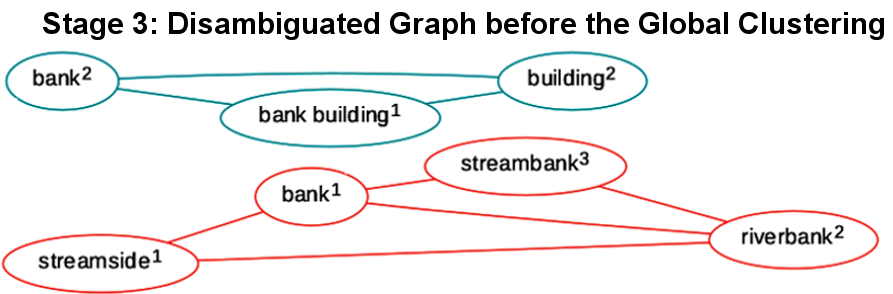
\includegraphics[width=1\textwidth]{figures/stages3}	
%\end{frame}
%
%
%\begin{frame}{Synset induction}
%
%  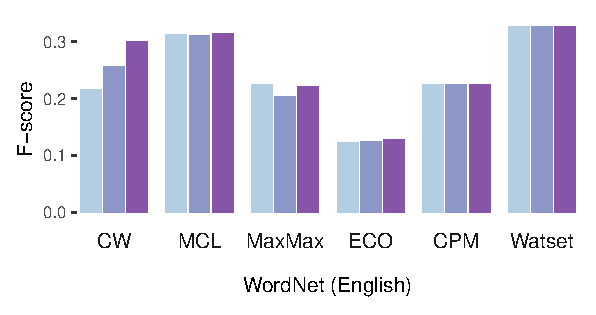
\includegraphics[width=0.49\textwidth]{figures/edges-en-wordnet}  
%  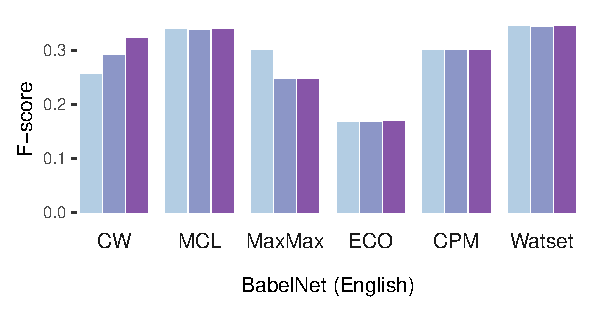
\includegraphics[width=0.49\textwidth]{figures/edges-en-babelnet}
%
%  \pause    
%  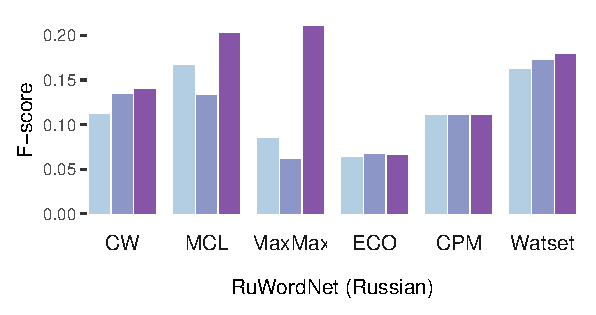
\includegraphics[width=0.49\textwidth]{figures/edges-ru-rwn}     
%  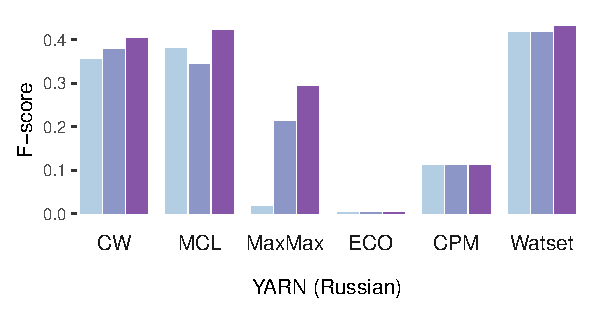
\includegraphics[width=0.49\textwidth]{figures/edges-ru-yarn}     
%	
%\end{frame}
%




\begin{frame}{Semantic roles  }

\begin{itemize}
\item Semantic frame ``Abandonment'' from FrameNet 	
\end{itemize}


	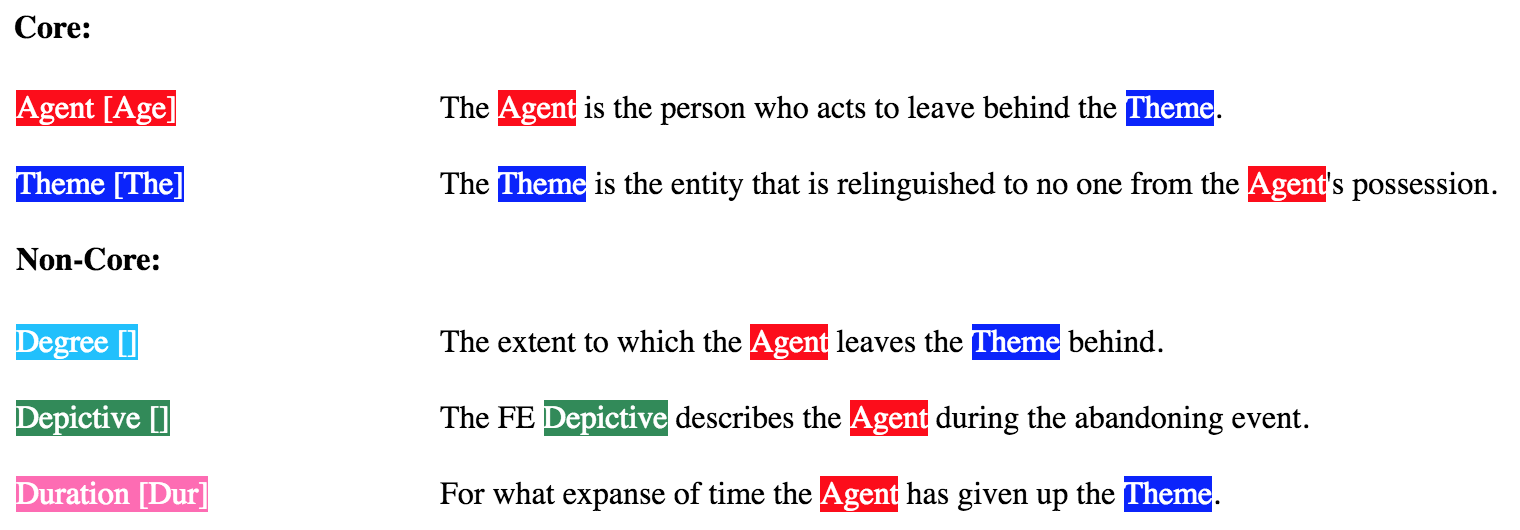
\includegraphics[width=1.0\textwidth]{figures/roles}
\end{frame}



\begin{frame}{Semantic classes  }

\begin{itemize}
\item A semantic class contains words that share a \textbf{semantic feature}.
\item Examples of \textbf{concrete semantic classes}:
\begin{itemize}
\item  people
\item  plants
\item  animals
\item  materials
\item  programming languages
\end{itemize}

\item Examples of \textbf{abstract semantic classes}: 

\begin{itemize}
\item qualities
\item actions
\item processes
\end{itemize}


  	
\end{itemize}


\end{frame}


	
\begin{frame}{Sample of induced \alert{sense inventory}}


\begin{table}
\centering
\scriptsize
\begin{tabular}{l|p{6cm}|p{2.5cm}} 
\bf Word Sense & \bf Local Sense Cluster: Related Senses & \bf Hypernyms \\
\toprule
 \alert{mango\#0} &  peach\#1, grape\#0, plum\#0, apple\#0, apricot\#0, watermelon\#1, banana\#1, coconut\#0, pear\#0, fig\#0, melon\#0,  \alert{\textbf{mangosteen\#0}}, ... & fruit\#0, food\#0, ... \\
 
\midrule
\alert{apple\#0} & mango\#0, pineapple\#0, banana\#1, melon\#0, grape\#0, peach\#1, watermelon\#1, apricot\#0, cranberry\#0, pumpkin\#0, \alert{\textbf{mangosteen\#0}}, ... & fruit\#0, crop\#0,  ... \\

\midrule
Java\#1 & C\#4, Python\#3, Apache\#3, Ruby\#6, Flash\#1, C++\#0, SQL\#0, ASP\#2, Visual Basic\#1, CSS\#0, Delphi\#2, MySQL\#0, Excel\#0, Pascal\#0, ... & programming language\#3, language\#0, ... \\

\midrule
Python\#3 & PHP\#0, Pascal\#0, Java\#1, SQL\#0, Visual Basic\#1, C++\#0, JavaScript\#0, Apache\#3, Haskell\#5, .NET\#1, C\#4, SQL Server\#0, ... & language\#0, technology\#0, ... \\

\end{tabular}


\end{table}


\note{ entries  representing ``fruits'' and ``programming language'' senses. Each word sense $s$ is represented with a list of related senses $\mathcal{N}(s)$ and the list of hypernyms $\mathcal{H}(s)$. The hypernyms can be used as human-interpretable sense labels of the sense clusters. One sense $s$, such as ``apple\#0'', can appear in multiple entries.}

\end{frame}


\begin{frame}{Sample of induced \alert{semantic classes}}


\begin{table}
\centering
\scriptsize
\begin{tabular}{l|p{2.5in}|p{1in}} 
\bf ID &  \bf Global Sense Cluster: Semantic Class & \bf Hypernyms \\ 

\toprule

1 & peach\#1, banana\#1, pineapple\#0, berry\#0, blackberry\#0, grapefruit\#0, strawberry\#0, blueberry\#0, \alert{mango\#0}, grape\#0, melon\#0, orange\#0, pear\#0, plum\#0, raspberry\#0, watermelon\#0, \alert{apple\#0}, apricot\#0, watermelon\#0, pumpkin\#0, berry\#0, \alert{\textbf{mangosteen\#0}}, ...  & vegetable\#0, fruit\#0, crop\#0, ingredient\#0, food\#0, $\cdot$ \\ 

\midrule

2  & C\#4, Basic\#2, Haskell\#5, Flash\#1, \alert{Java\#1}, Pascal\#0, Ruby\#6, PHP\#0, Ada\#1, Oracle\#3, \alert{Python\#3}, Apache\#3, Visual Basic\#1, ASP\#2, Delphi\#2, SQL Server\#0, CSS\#0, AJAX\#0, JavaScript\#0, SQL Server\#0, Apache\#3, Delphi\#2, Haskell\#5, .NET\#1, CSS\#0, ... & programming language\#3, technology\#0, language\#0, format\#2, app\#0
\end{tabular}

\note{Sample of the induced  sense clusters representing ``fruits'' and ``programming language'' semantic classes. Similarly to the induced word senses, the semantic classes are labeled with hypernyms. In contrast to the induced word senses, which represent a local clustering of word senses (related to a given word) semantic classes represent a global sense clustering of word senses. One sense $c$, such as ``apple\#0'', can appear only in a single cluster.}


\end{table}

\end{frame}


%
%\begin{frame}{Induction of  semantic classes}
%
%Examples of semantic classes:
%
%\begin{table}[ht]
%\centering
%\scriptsize
%\begin{tabular}{l|p{6cm}|p{3.5cm}} 
%
%\bf ID &  \bf Sense Cluster & \bf Hypernyms \\ \hline
%& &  \\
%1 & peach\#1, banana\#1, pineapple\#0, berry\#0, blackberry\#0, grapefruit\#0, strawberry\#0, blueberry\#0, grape\#0, melon\#0, orange\#0, pear\#0, plum\#0, raspberry\#0, watermelon\#0, apple\#0, apricot\#0, ...  &  fruit\#0, crop\#0, ingredient\#0, food\#0, $\cdot$ \\ & &  \\ \hline
%& &  \\
%2  & C\#4, Basic\#2, Haskell\#5, Flash\#1, Java\#1, Pascal\#0, Ruby\#6, PHP\#0, Ada\#1, Oracle\#3, Python\#3, Apache\#3, Visual Basic\#1, ASP\#2, Delphi\#2, SQL Server\#0, CSS\#0, AJAX\#0, the Java\#0, ... & programming language\#3, technology\#0, language\#0, format\#2, app\#0 
%\end{tabular}
%\end{table}
%
%	
%\end{frame}



\begin{frame}{Induction of  semantic classes}
	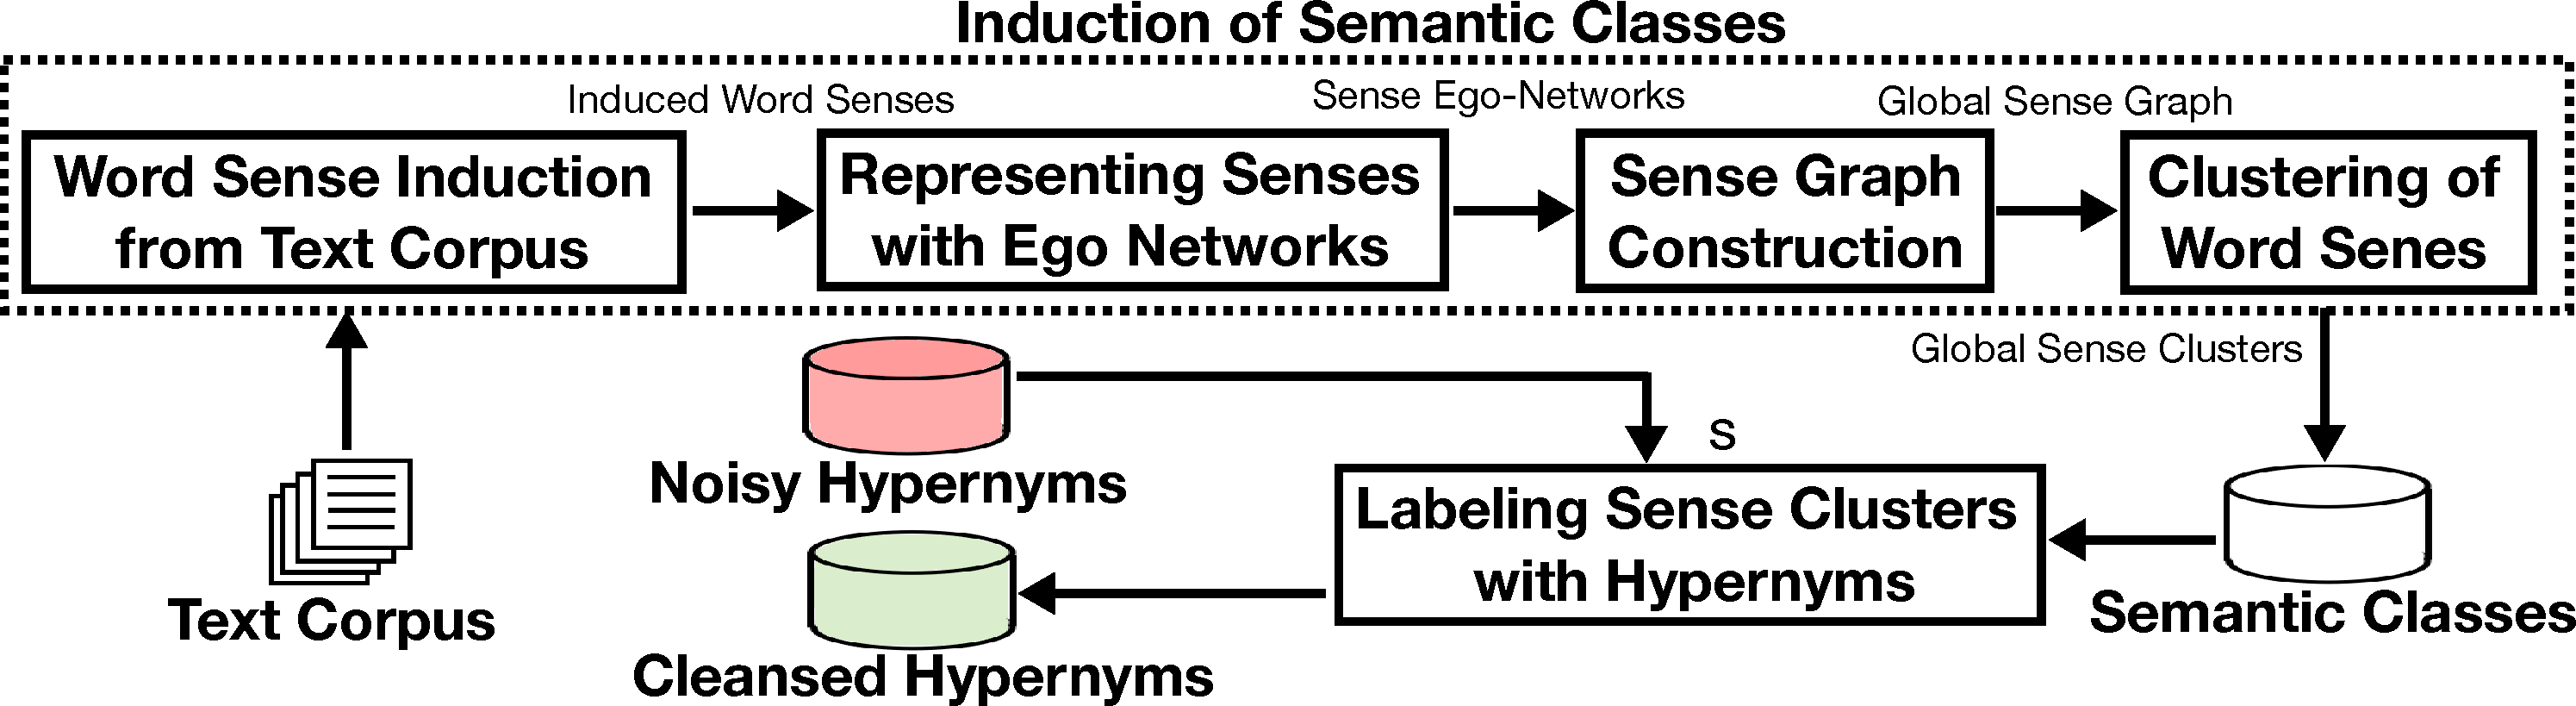
\includegraphics[width=1.0\textwidth]{figures/outline-semantic-classes}
\end{frame}




\begin{frame}{Induction of sense semantic classes}

Filtering noisy hypernyms with semantic classes \textbf{LREC'18}~\cite{panchenko:2018:SemanticClasses}: 

	\centering 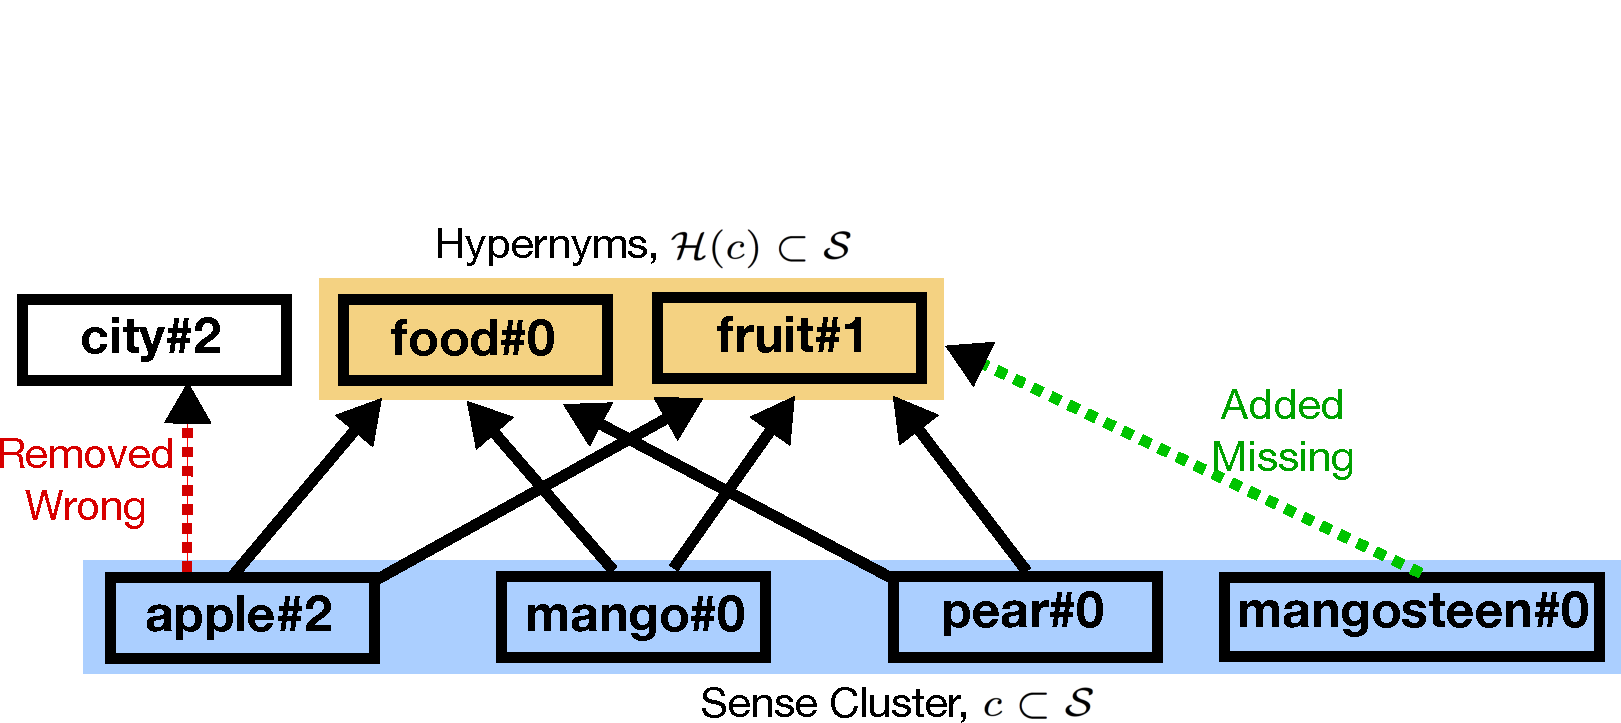
\includegraphics[width=1.0\textwidth]{figures/coset}
	
\end{frame}



\begin{frame}{Global sense clustering}


\vspace{-10pt}
{\footnotesize \underline{\url{http://panchenko.me/data/joint/nodes20000-layers7}}}


\begin{center}
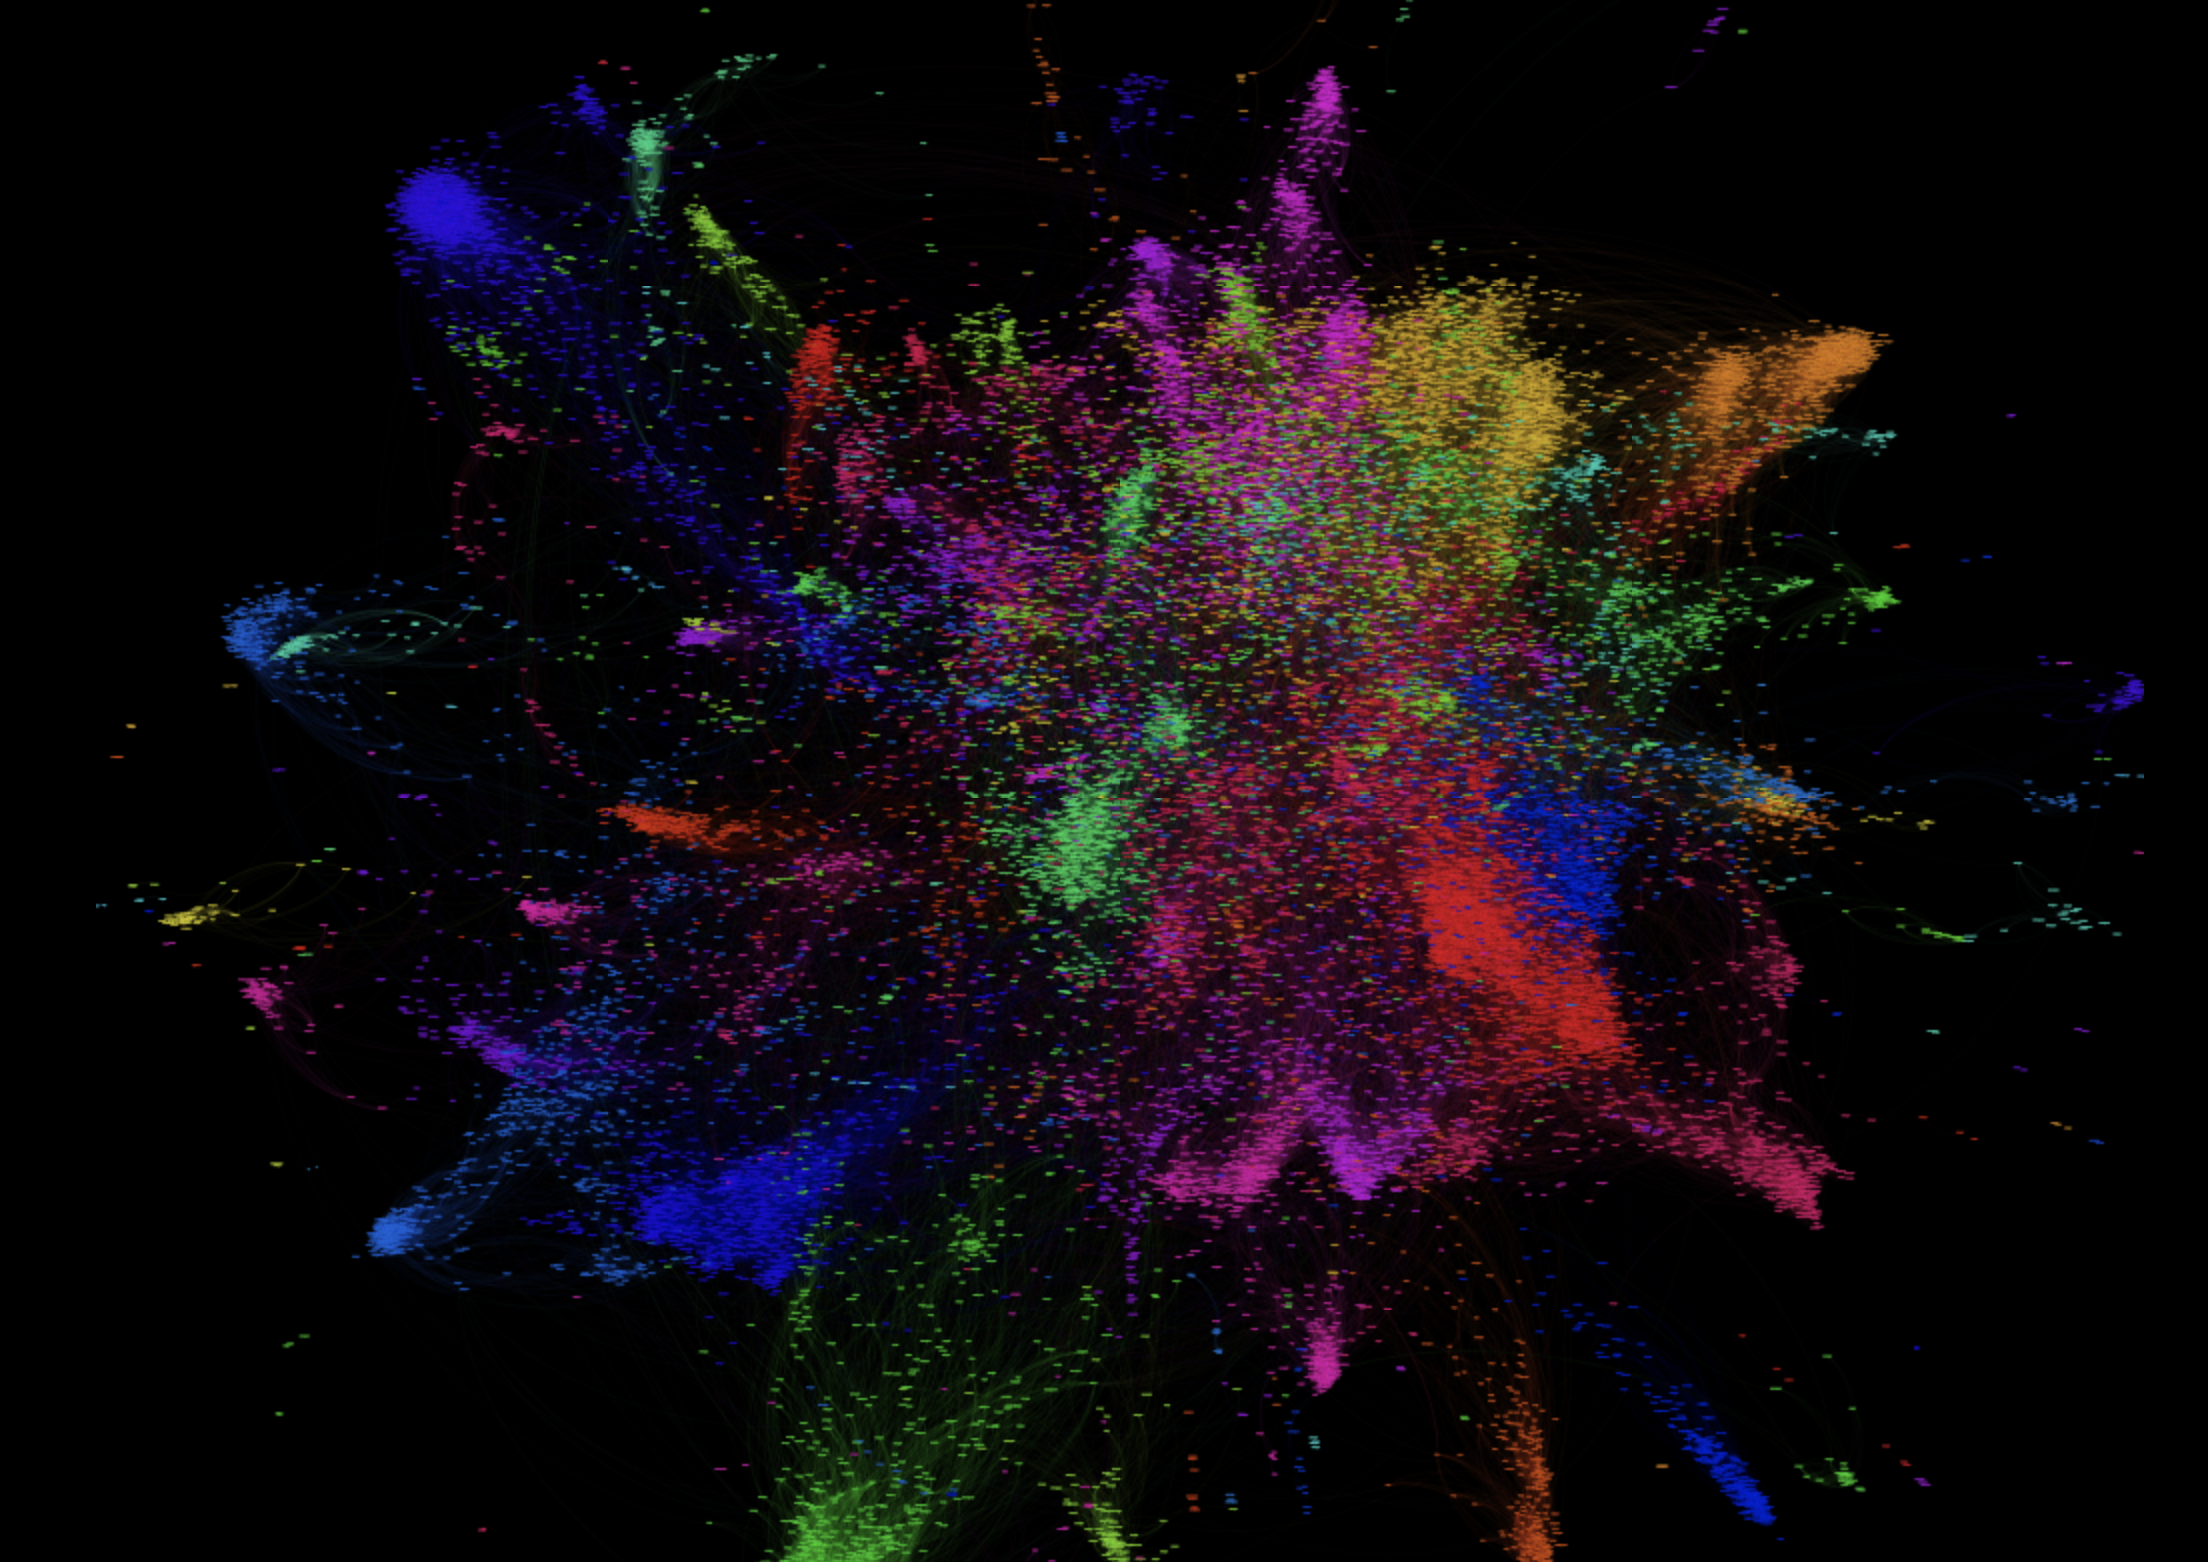
\includegraphics[width=.75\textwidth]{figures/structure}
\end{center}

\end{frame}



\begin{frame}{Global sense clustering}

\begin{center}
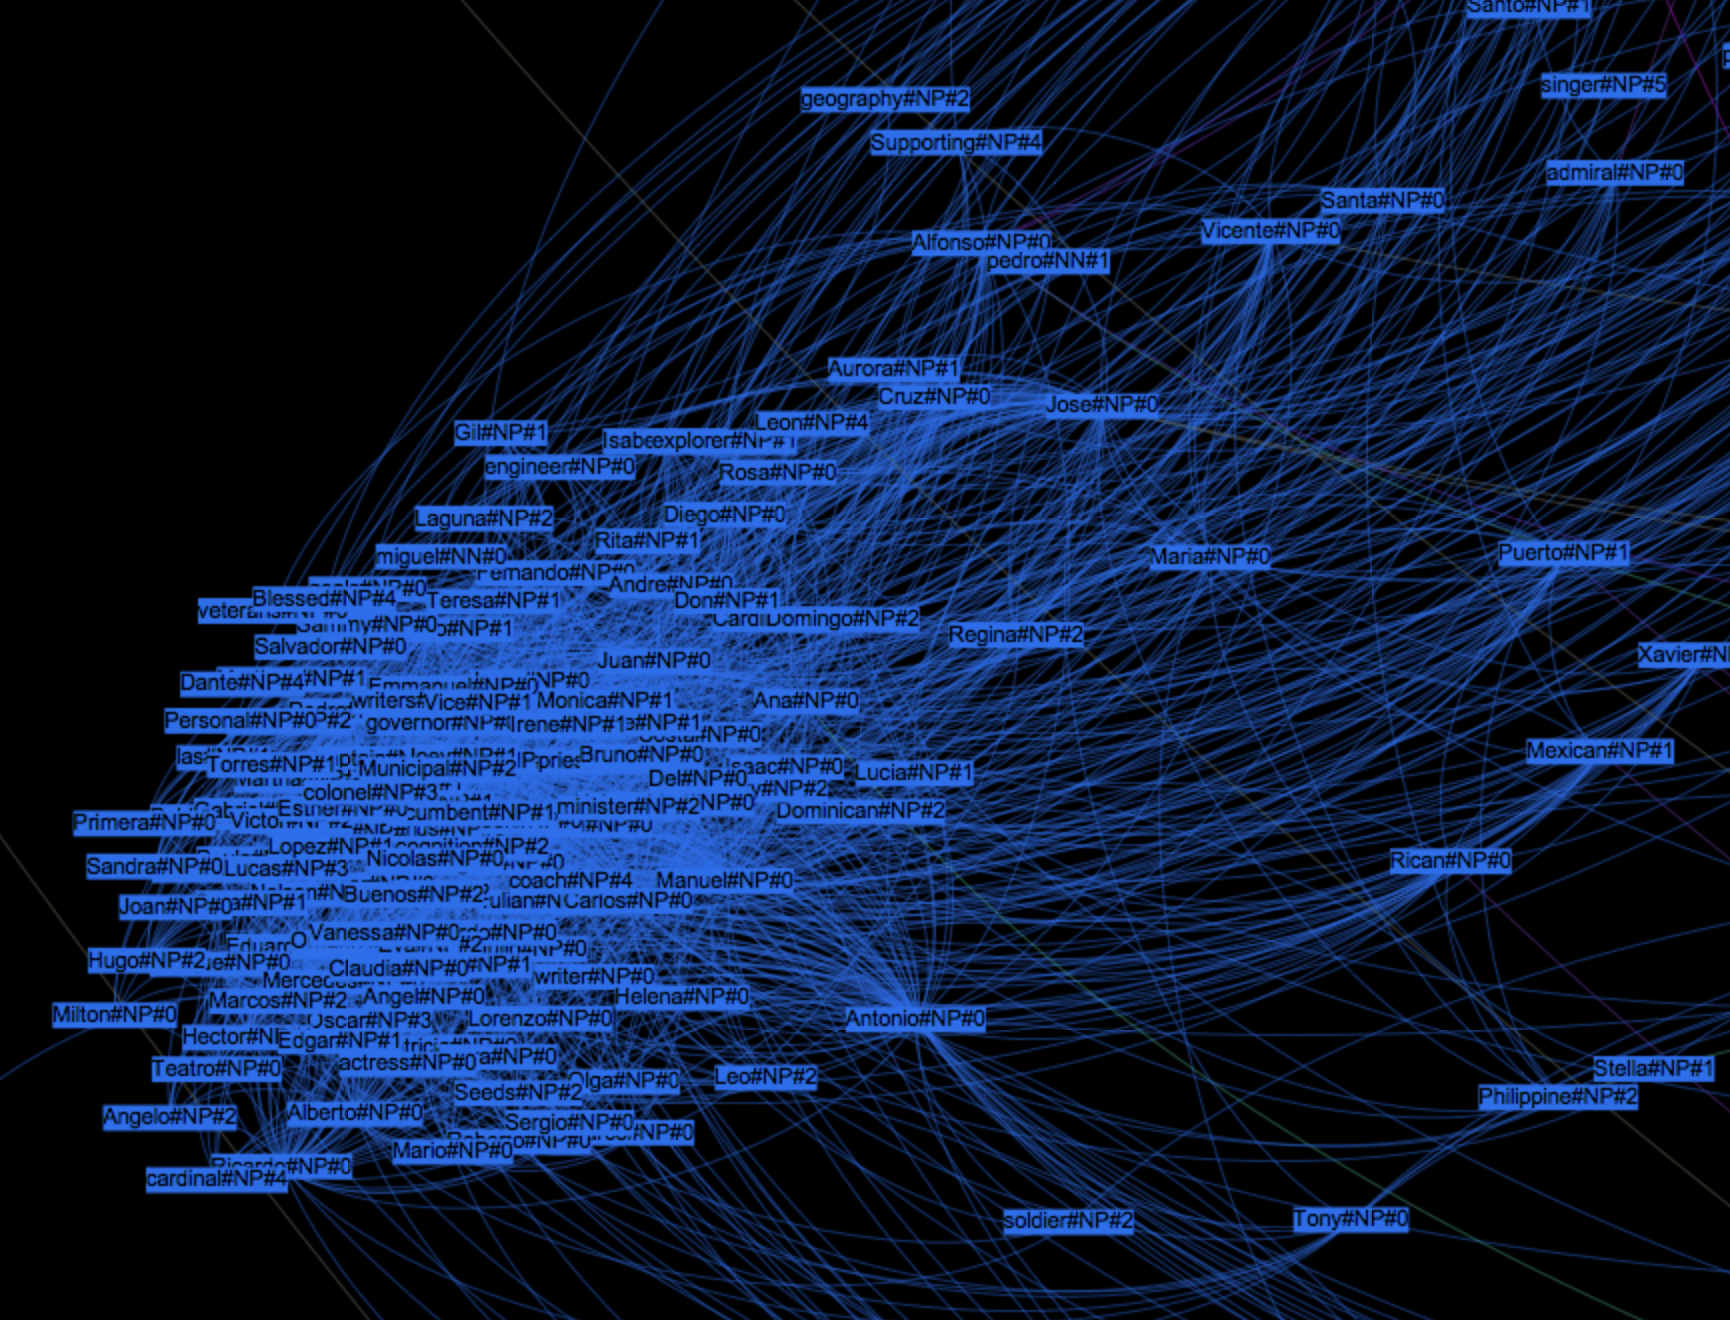
\includegraphics[width=.75\textwidth]{figures/structure1}
\end{center}

\end{frame}



\begin{frame}{Induction of sense semantic classes}

Filtering of a noisy hypernymy database with semantic classes.  \textbf{LREC'18}~\cite{panchenko:2018:SemanticClasses}

\begin{table}
\scriptsize
\centering
\resizebox{1.0\linewidth}{!}{
\begin{tabular}{l|c|c|c}
 & \textbf{Precision} & \textbf{Recall} & \textbf{F-score} \\ \hline
Original Hypernyms  (Seitner et al., 2016) & $0.475$ & $0.546$ & $0.508$ \\
Semantic Classes (coarse-grained) & $\mathbf{0.541}$ & $\mathbf{0.679}$ & $\mathbf{0.602}$ \\
\end{tabular}
}
\end{table}
	
\end{frame}





\section{Making induced senses interpretable}


\begin{frame}{ Making induced senses interpretable }

\vspace{-1em}

\textbf{Knowledge-based} sense representations are \alert{\textbf{interpretable}}
%\begin{columns}
%\begin{column}{0.70\textwidth}  %%<--- here
	\begin{center}
	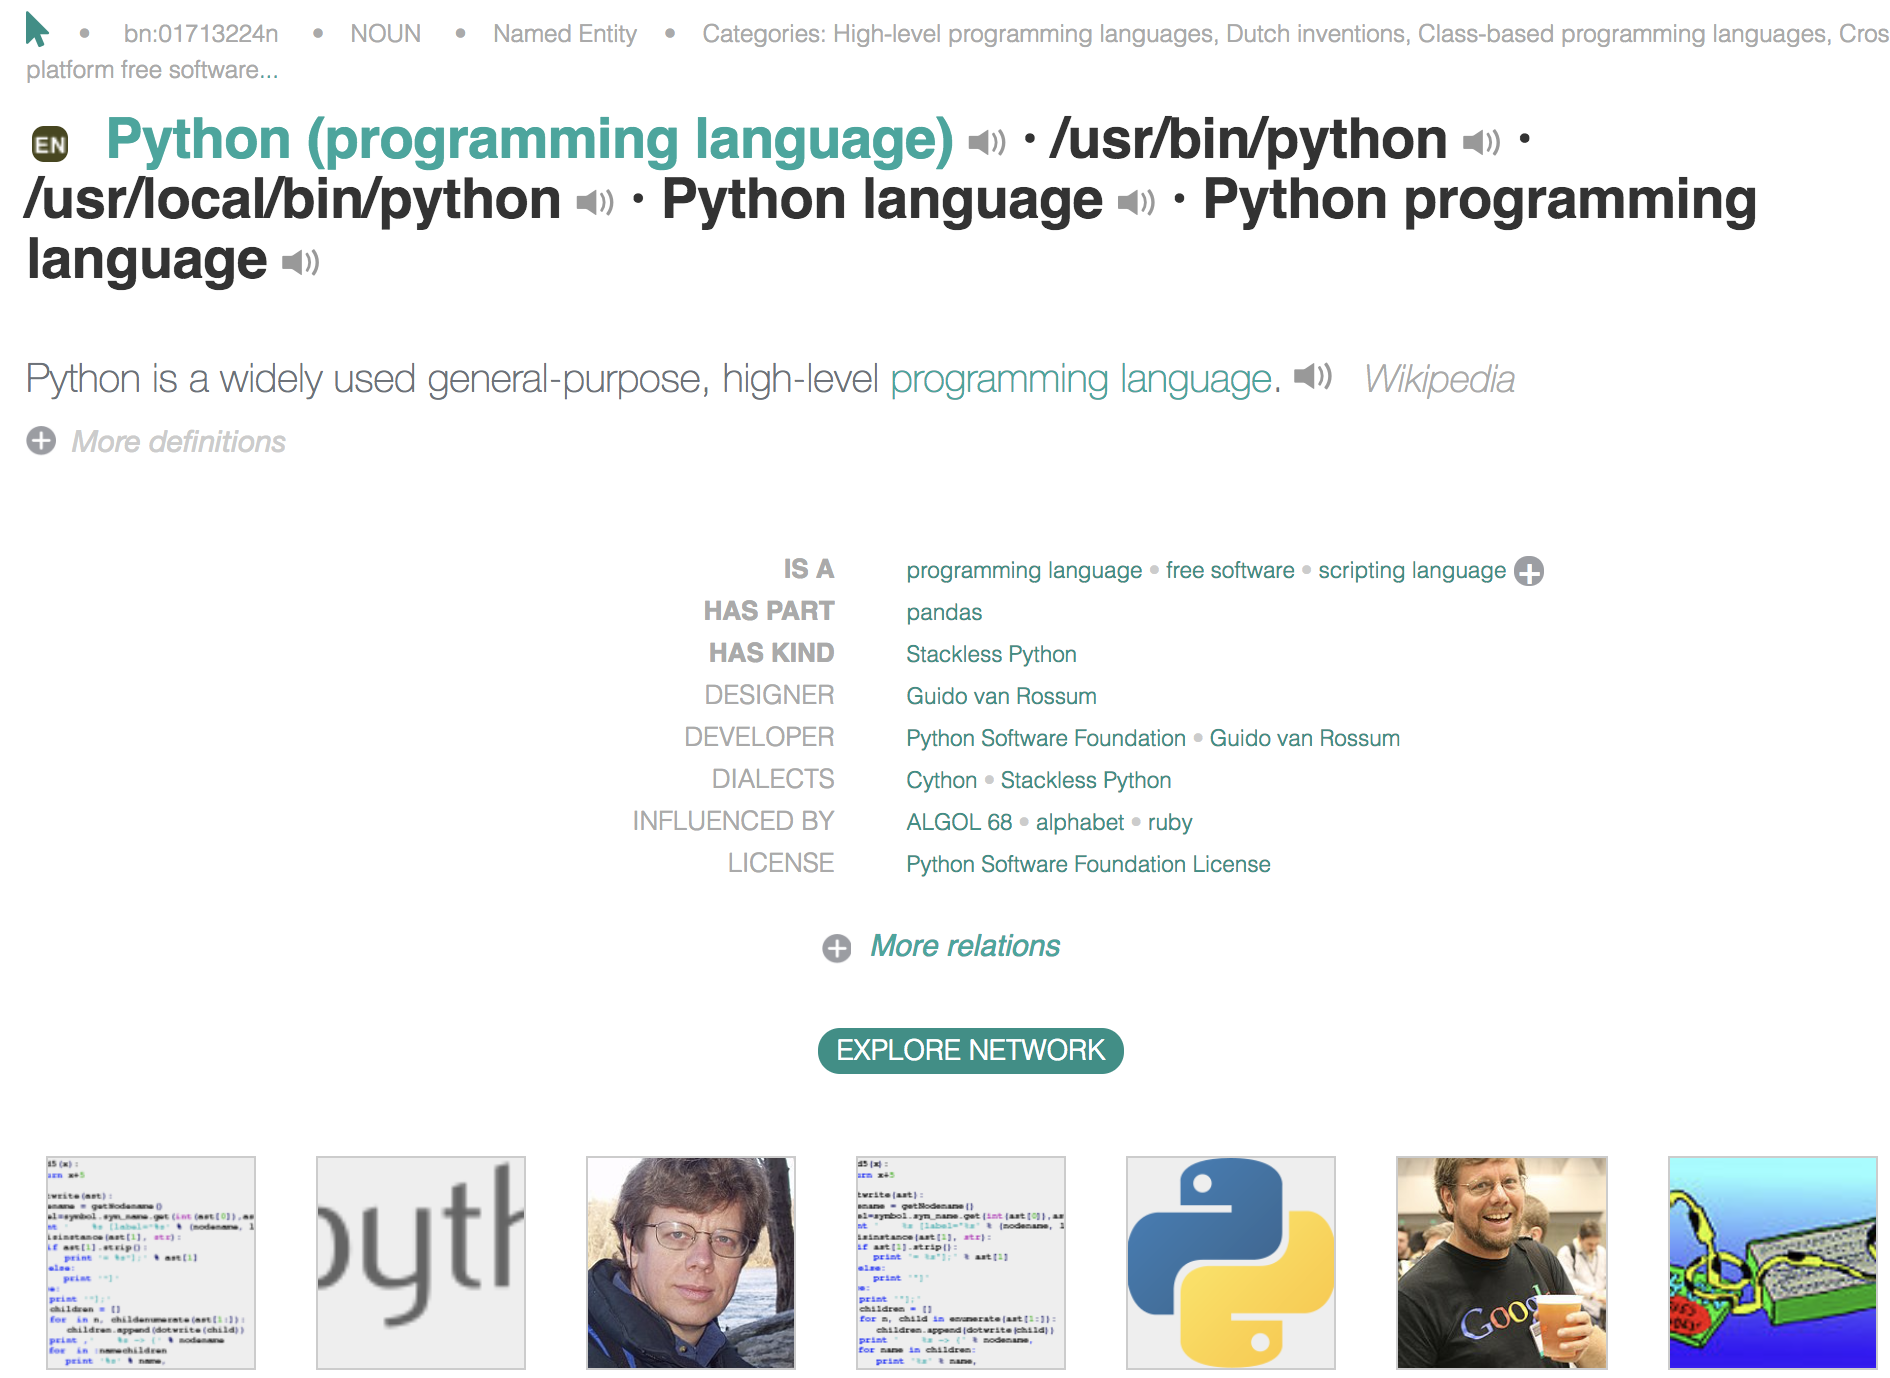
\includegraphics[width=0.75\textwidth]{babelnet}
	\end{center}

%\end{column}
%\begin{column}{0.30\textwidth}
%Knowledge-based sense representations are \alert{\textbf{interpretable}}:
%		 \pause
%	\begin{itemize}
%		\item \textbf{synonyms},
%		\item \textbf{hypernyms},
%		\item \textbf{images},
%		\item \textbf{definitions},
%		\item ...  
%	\end{itemize}
%\end{column}
%\end{columns}

\end{frame}


\begin{frame}{ Making induced senses interpretable }

\vspace{-1em}
Most \textbf{knowledge-free} sense representations are 
\alert{\textbf{uninterpretable}}

	\begin{center}
	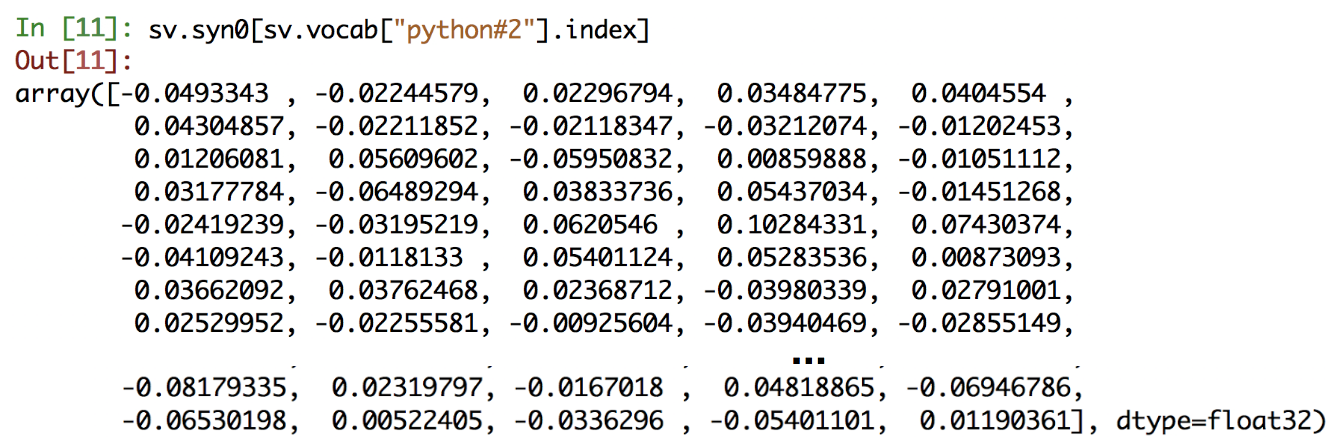
\includegraphics[width=1.\textwidth]{numpy}
	\end{center}	

\end{frame}


\begin{frame}{ Making induced senses interpretable }

\vspace{-1em}
	\begin{center}
	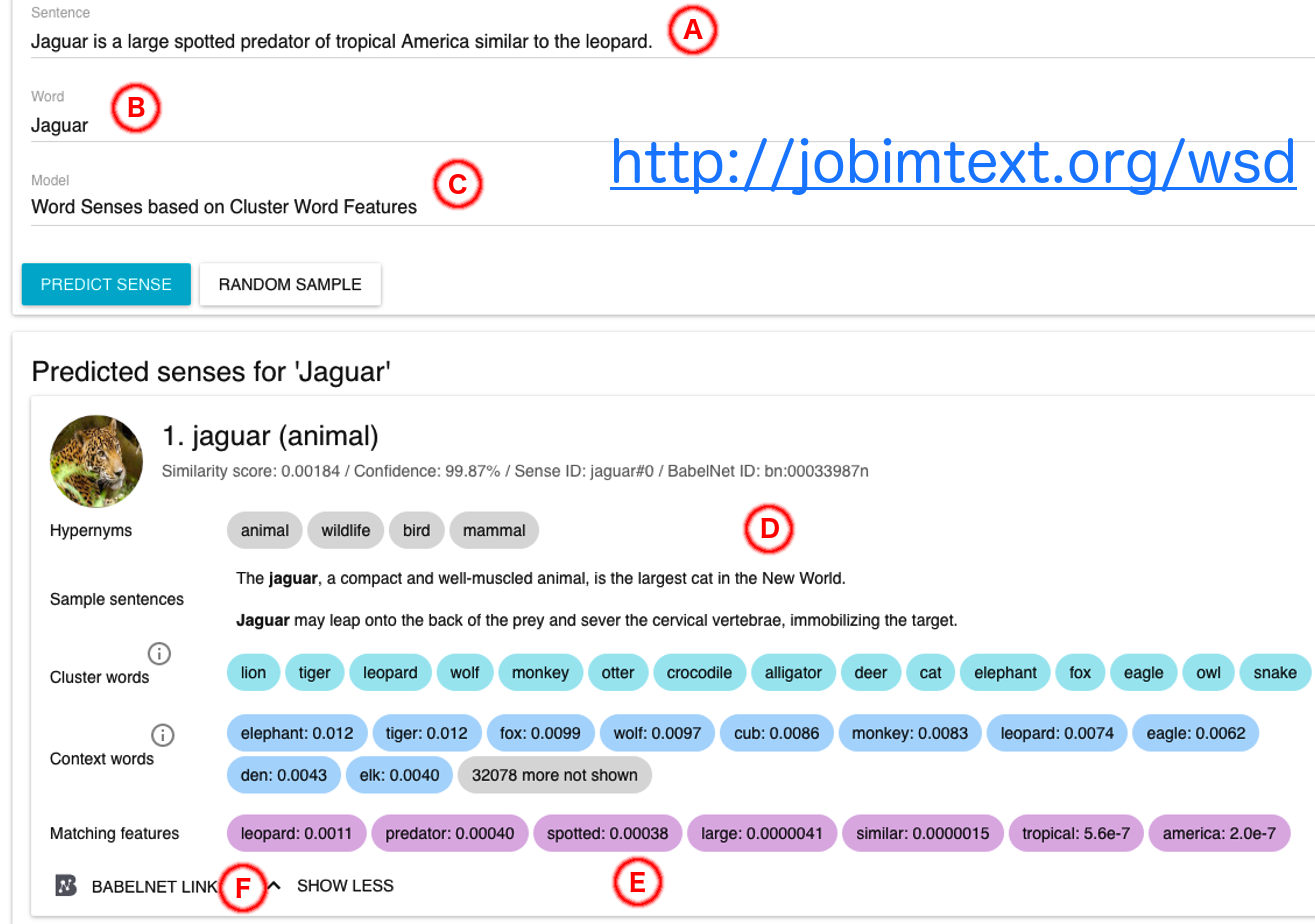
\includegraphics[width=0.85\textwidth]{emnlp_single}
	\end{center}	
\end{frame}


\begin{frame}{ Making induced senses interpretable }

\vspace{-1em}
	\begin{center}
	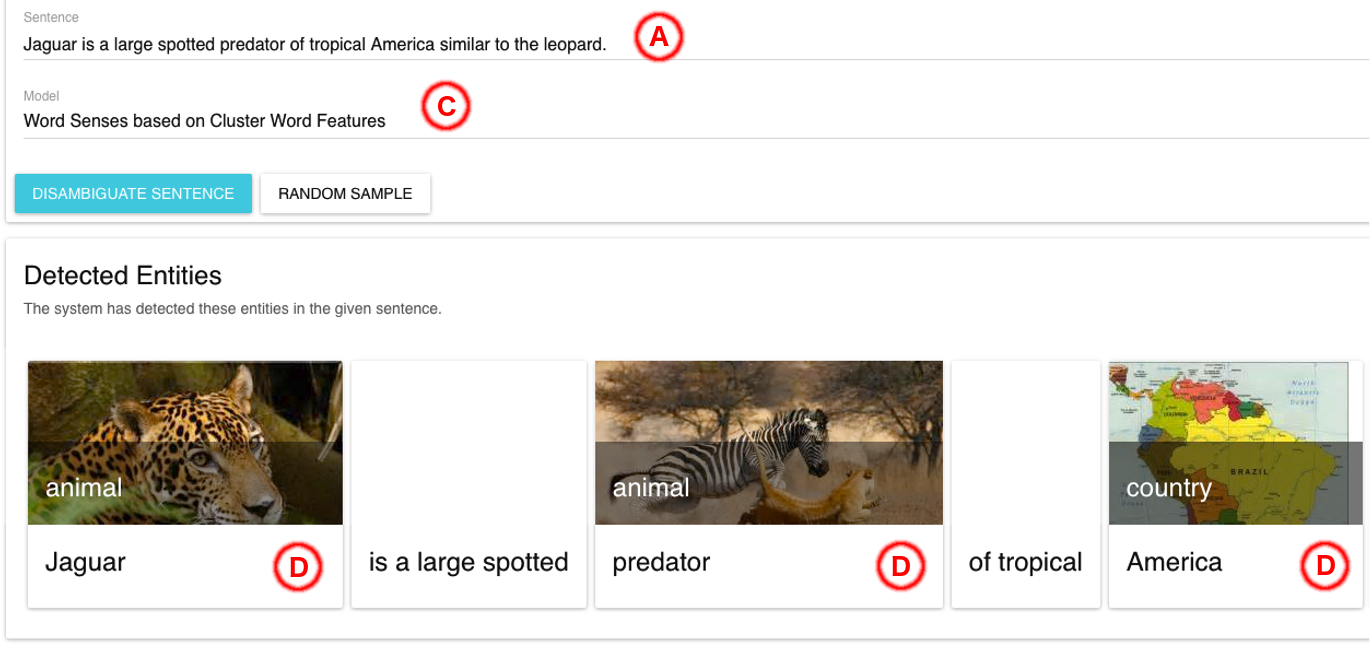
\includegraphics[width=1.05\textwidth]{emnlp_all}
	
	{\footnotesize Hypernymy prediction in context. \textbf{EMNLP'17}~\cite{panchenko-EtAl:2017:EMNLP2017Demos}}
	\end{center}	
	
	

	
\end{frame}



\begin{frame}{ Making induced senses interpretable }
	
	
\vspace{-1em}
	
\begin{itemize}
	\item \textbf{11.702 sentences}, \textbf{863 words} with \textbf{avg.polysemy of 3.1}.   
\end{itemize}  

\begin{center}
	
\begin{tabular}{llcc}

\multicolumn{2}{c}{\bf WSD Model} & \multicolumn{2}{c}{\bf Accuracy}  \\
Inventory & Features & Hypers &  HyperHypers  \\ \toprule

Word Senses & Random  & 0.257 & 0.610 \\
Word Senses & MFS  & 0.292 & 0.682 \\
Word Senses & Cluster Words & 0.291 & 0.650 \\
Word Senses & Context Words & \underline{\textbf{0.308}} & \underline{\textbf{0.686}} \\
\hline \pause
Super Senses & Random & 0.001 & 0.001 \\
Super Senses & MFS & 0.001 & 0.001 \\
Super Senses & Cluster Words & \textbf{0.174} & \textbf{0.365} \\
Super Senses & Context Words & 0.086 & 0.188 \\

\end{tabular}

\end{center}
	
\end{frame}


\section{Linking induced senses to resources}

\begin{frame}{ Linking induced senses to resources }
	
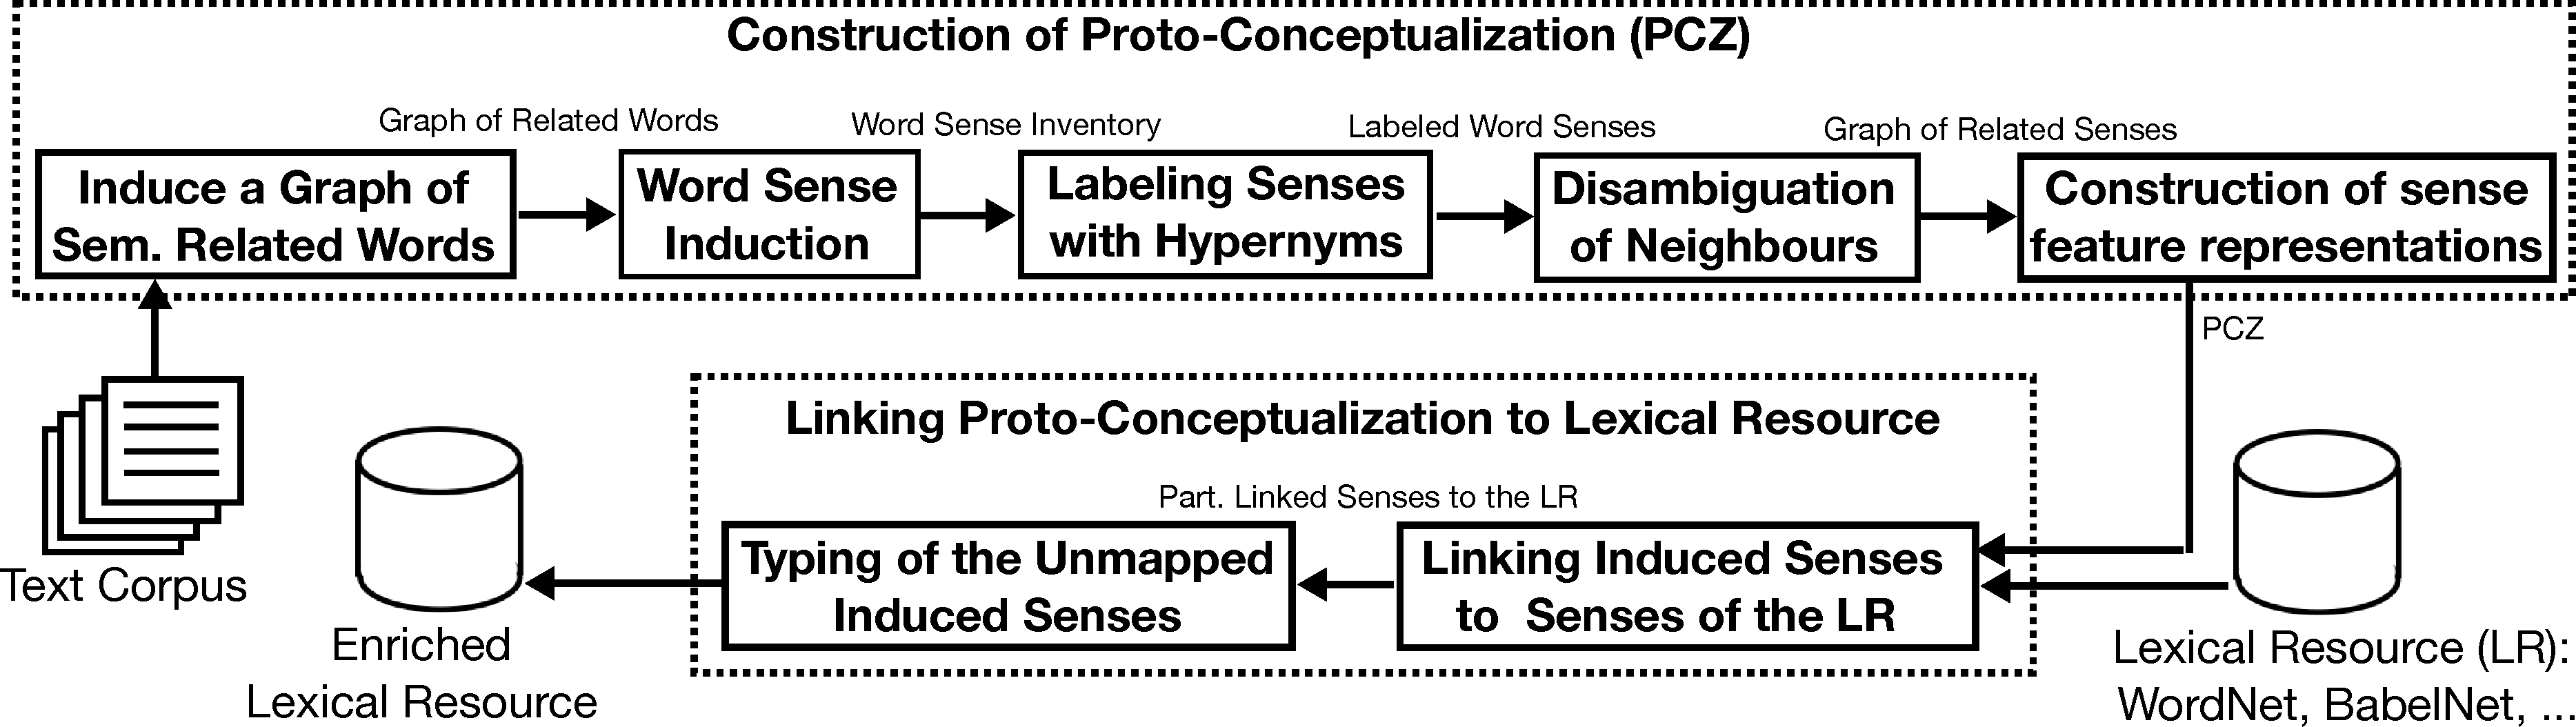
\includegraphics[width=1.05\textwidth]{linking-outline}
\vspace{2em}

\textbf{LREC'16}~\cite{panchenko2016best}, \textbf{ISWC'16}~\cite{faralli2016linked}, \textbf{SENSE@EACL'17}~\cite{panchenko-EtAl:2017:SENSE2017}, \textbf{NLE'18}~\cite{biemann2018framework}

\end{frame}

\begin{frame}{ Linking induced senses to resources }
\vspace{-1em}
%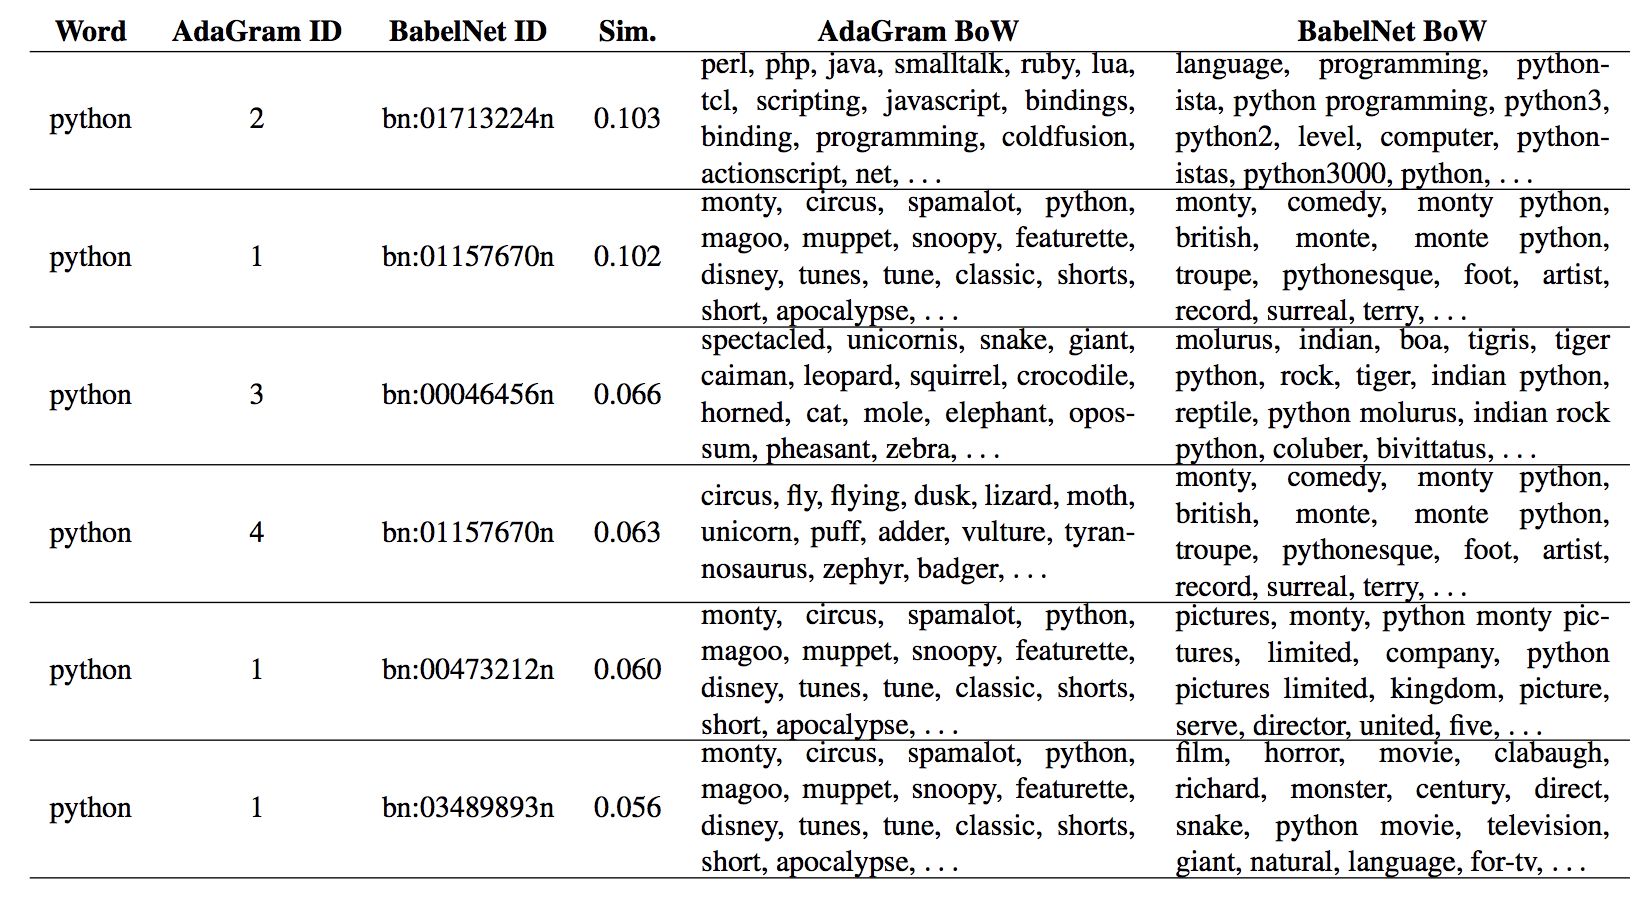
\includegraphics[width=1.05\textwidth]{mapping}
\begin{table}

\tiny  
\begin{center}
\begin{tabular}{ccc p{3cm} p{3cm}}

\bf Word & \bf AdaGram & \bf BabelNet & \bf AdaGram BoW & \bf BabelNet BoW  \\
\hline

python & 2 & bn:01713224n   & perl, php, java, smalltalk, ruby, lua, tcl, scripting, javascript, bindings, binding, programming, coldfusion, actionscript, net, $\ldots$ &  language, programming, pythonista,  python programming, python3, python2, level, computer, pythonistas, python3000, \\ \hline

python & 1 & bn:01157670n & monty, circus, spamalot, python, magoo, muppet, snoopy, featurette, disney, tunes, tune, classic, shorts, short, apocalypse, $\ldots$ &  monty, comedy, monty python, british, monte, monte python, troupe, pythonesque, foot, artist, record, surreal, terry, $\ldots$ \\ \hline

python & 3 & bn:00046456n  & spectacled, unicornis, snake, giant, caiman, leopard, squirrel, crocodile, horned, cat, mole, elephant, opossum, pheasant, $\ldots$ &  molurus, indian, boa, tigris, tiger python, rock, tiger, indian python, reptile, python molurus, indian rock python, coluber, $\ldots$ \\ \hline

python & 4 & bn:01157670n & circus, fly, flying, dusk, lizard, moth, unicorn, puff, adder, vulture, tyrannosaurus, zephyr, badger, $\ldots$ & monty, comedy, monty python, british, monte, monte python, troupe, pythonesque, foot, artist, record, surreal, terry, $\ldots$ \\ \hline

python & 1 & bn:00473212n  & monty, circus, spamalot, python, magoo, muppet, snoopy, featurette, disney, tunes, tune, classic, shorts, short, apocalypse, $\ldots$ &  pictures, monty, python monty pictures, limited, company, python pictures limited, kingdom, picture, serve, director, $\ldots$ \\ \hline

python & 1 & bn:03489893n  & monty, circus, spamalot, python, magoo, muppet, snoopy, featurette, disney, tunes, tune, classic, shorts, short, apocalypse, $\ldots$ &  film, horror, movie, clabaugh, richard, monster, century, direct, snake, python movie, television, giant, natural, language, for-tv, $\ldots$ 
\end{tabular}
\end{center}
\end{table}
	
	
\end{frame}


\begin{frame}{Linking induced senses to resources }


\begin{table}
\tiny
\begin{tabular}{l|p{9cm}} 
\bf Model & \bf Sense Representation \\ \hline
\textbf{WordNet}  &  memory, device, floppy, disk, hard, disk, disk, computer, science, computing, diskette, fixed, disk, floppy, magnetic, disc, magnetic, disk, hard, disc,      storage, device \\ \\ \hline 
\textbf{WordNet + Linked} & recorder, disk, floppy, console, diskette, handset, desktop, iPhone, iPod, HDTV, kit, RAM, Discs, Blu-ray, computer, GB, microchip, site, cartridge,          printer, tv, VCR, Disc, player, LCD, software, component, camcorder, cellphone, card, monitor, display, burner, Web, stereo, internet, model, iTunes,         turntable, chip, cable, camera, iphone, notebook, device, server, surface, wafer, page, drive, laptop, screen, pc, television, hardware, YouTube, dvr,        DVD, product, folder, VCR, radio, phone, circuitry, partition, megabyte, peripheral, format, machine, tuner, website, merchandise, equipment, gb, discs,      MP3, hard-drive, piece, video, storage device, memory device, microphone, hd, EP, content, soundtrack, webcam, system, blade, graphic, microprocessor,        collection, document, programming, battery, keyboard, HD, handheld, CDs, reel, web, material, hard-disk, ep, chart, debut, configuration, recording,          album, broadcast, download, fixed disk, planet, pda, microfilm, iPod, videotape, text, cylinder, cpu, canvas, label, sampler, workstation, electrode,         magnetic disc, catheter, magnetic disk, Video, mobile, cd, song, modem, mouse, tube, set, ipad, signal, substrate, vinyl, music, clip, pad, audio,            compilation, memory, message, reissue, ram, CD, subsystem, hdd, touchscreen, electronics, demo, shell, sensor, file, shelf, processor, cassette, extra,       mainframe, motherboard, floppy disk, lp, tape, version, kilobyte, pacemaker, browser, Playstation, pager, module, cache, DVD, movie, Windows, cd-rom, e-book, valve, directory, harddrive, smartphone, audiotape, technology, hard disk, show, computing, computer science, Blu-Ray, blu-ray, HDD, HD-DVD,            scanner, hard disc, gadget, booklet, copier, playback, TiVo, controller, filter, DVDs, gigabyte, paper, mp3, CPU, dvd-r, pipe, cd-r, playlist, slot, VHS,     film, videocassette, interface, adapter, database, manual, book, channel, changer, storage \\ 
\end{tabular}

\end{table}

	
\end{frame}



\begin{frame}{ Linking induced senses to resources }
		\vspace{2em}
		\centering
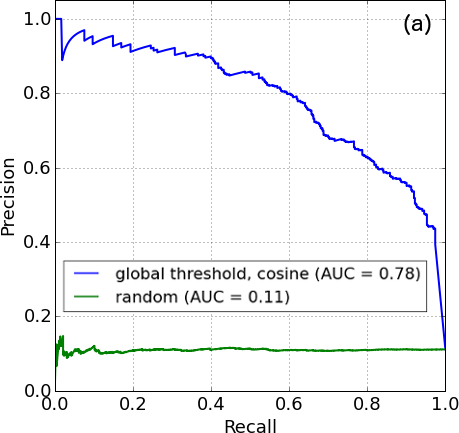
\includegraphics[width=0.41\textwidth]{precision-recall}

\includegraphics[width=0.06\textwidth]{filler}
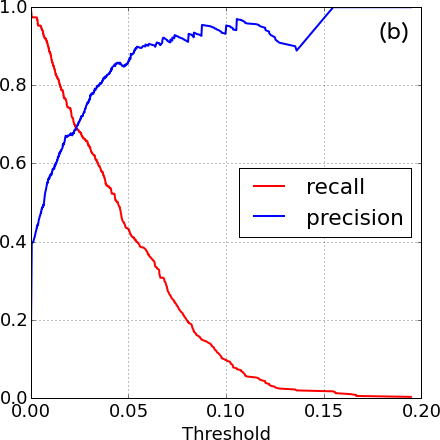
\includegraphics[width=0.40\textwidth]{pr-function-of-threshold}

\end{frame}

\begin{frame}{ Linking induced senses to resources }
\centering
Evaluation of enriched representations based on WSD:

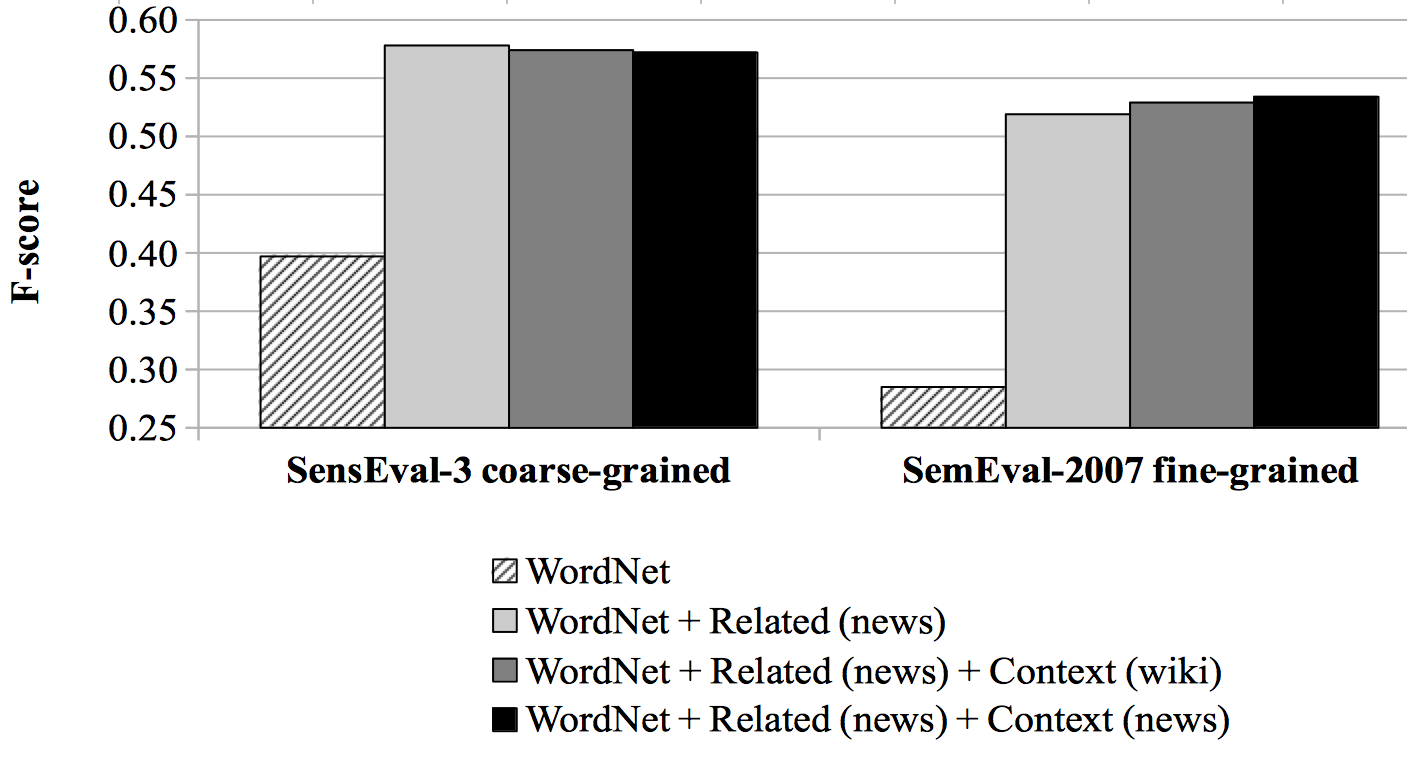
\includegraphics[width=1.0\textwidth]{topic-hist-4}

\end{frame}



\section{ $ $ $ $Word sense induction}

\subsection{}

%\begin{frame}{A shared task on WSI}
%  
%  \begin{itemize}
%  \item An \textbf{\alert{ACL SIGSLAV}} sponsored shared task on \textbf{word sense induction} (WSI) for the Russian language.
% \end{itemize} 
%  
%  \begin{itemize}
%    \item \textbf{More details}: \url{https://russe.nlpub.org/2018/wsi}
%     
%  \end{itemize}
%  
%  \begin{center}
%  	
\includegraphics[width=0.2\textwidth]{figures/acl}
%  \end{center}
%  
%%   \begin{center}
%%  	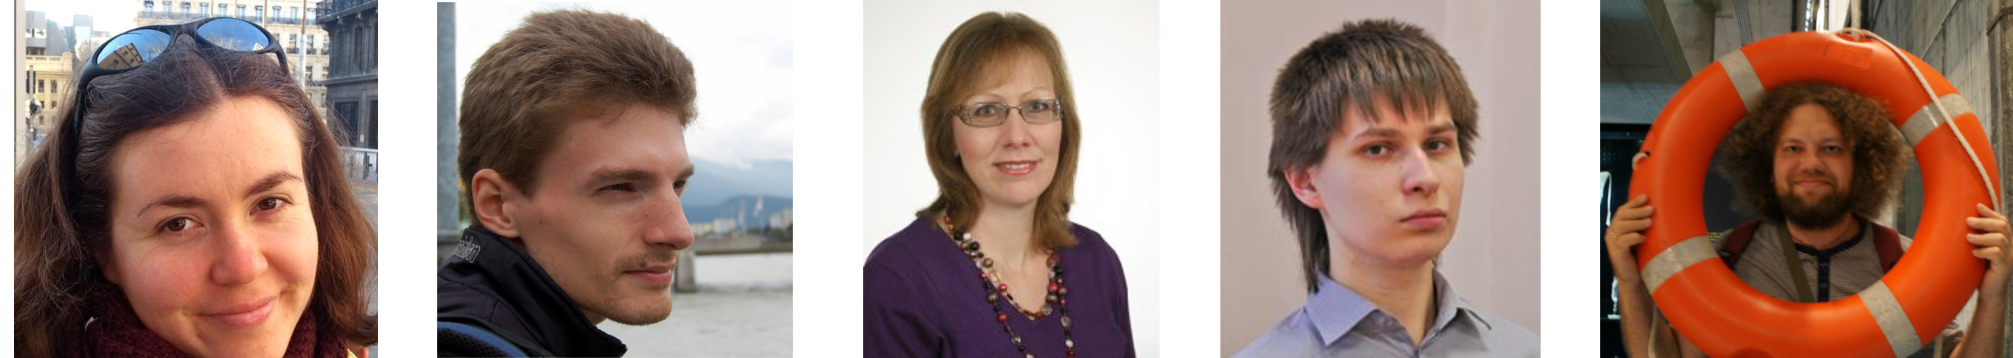
\includegraphics[width=0.99\textwidth]{figures/russe-team}
%%  \end{center}
%\end{frame}



\begin{frame}{A lexical sample WSI task}
  
  \begin{itemize}
  	\item \textbf{Target word}, e.g. ``bank''.
  	
  	\pause 
  	
  	\item \textbf{Contexts} where the word occurs, e.g.: 
  	\begin{itemize}
  	\item ``river \textbf{bank} is a slope beside a body of water''
  	\item ``\textbf{bank} is a financial institution that accepts deposits''
  	\item ``Oh, the \textbf{bank} was robbed. They took about a million dollars.''
  	\item ``\textbf{bank} of Elbe is a good and popular hangout spot complete with good food and fun''
  	\end{itemize}
  	
  	\pause 
  	
  	\item You need to \textbf{{group} the contexts by senses}:
  	\begin{itemize}
  	\item \textcolor{Cerulean}{``river \textbf{bank} is a slope beside a body of water''}
  	\item \textcolor{Cerulean}{``\textbf{bank} of Elbe is a good and popular hangout spot complete with good food and fun''}
  	\item \alert{``\textbf{bank} is a financial institution that accepts deposits''}
  	\item \alert{``Oh, the \textbf{bank} was robbed. They took about a million dollars.''}
  	\end{itemize}
  	 
  \end{itemize}
  
\end{frame}
%
%
%\begin{frame}{Dataset based on Wikipedia}
%
%{\centering
%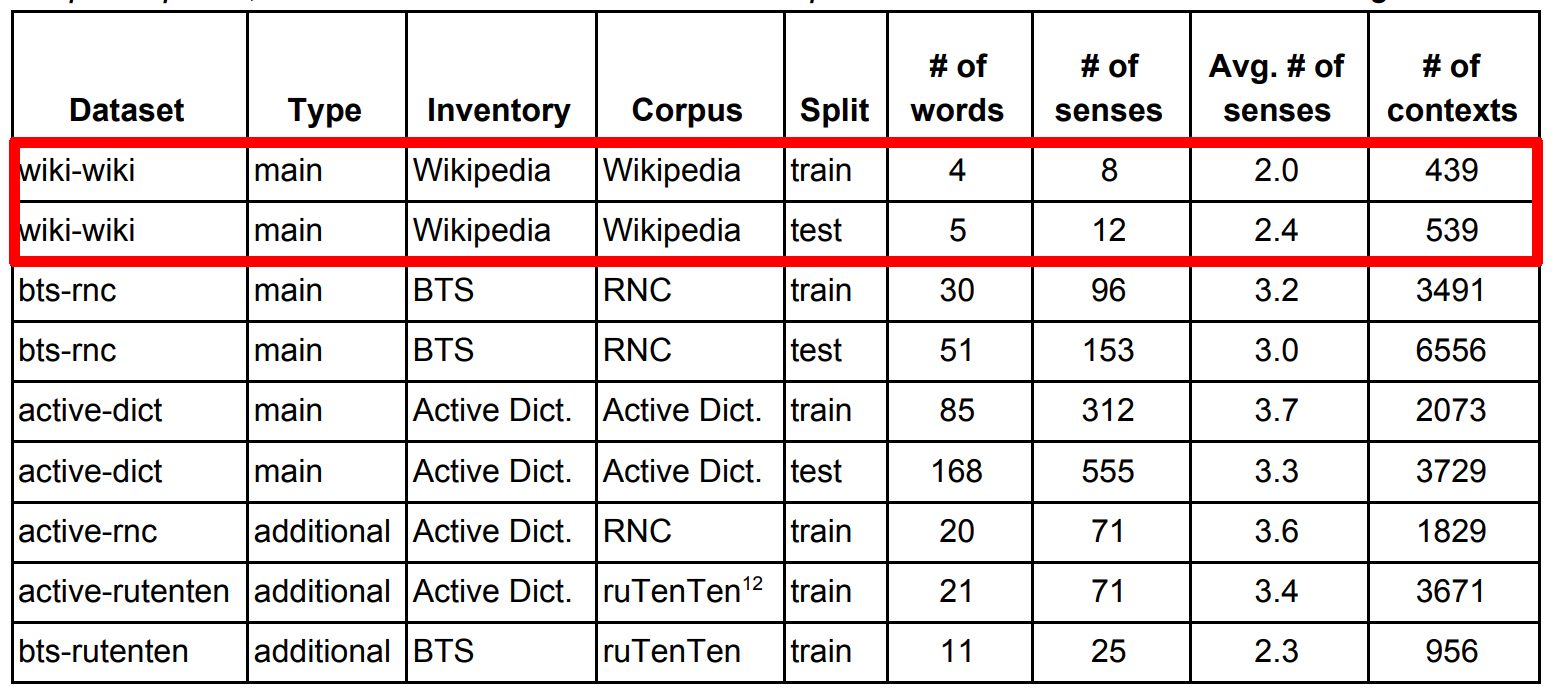
\includegraphics[width=1.0\textwidth]{figures/datasets1}
%}	
%\end{frame}
%
%
%\begin{frame}{Dataset based on RNC}
%
%{\centering
%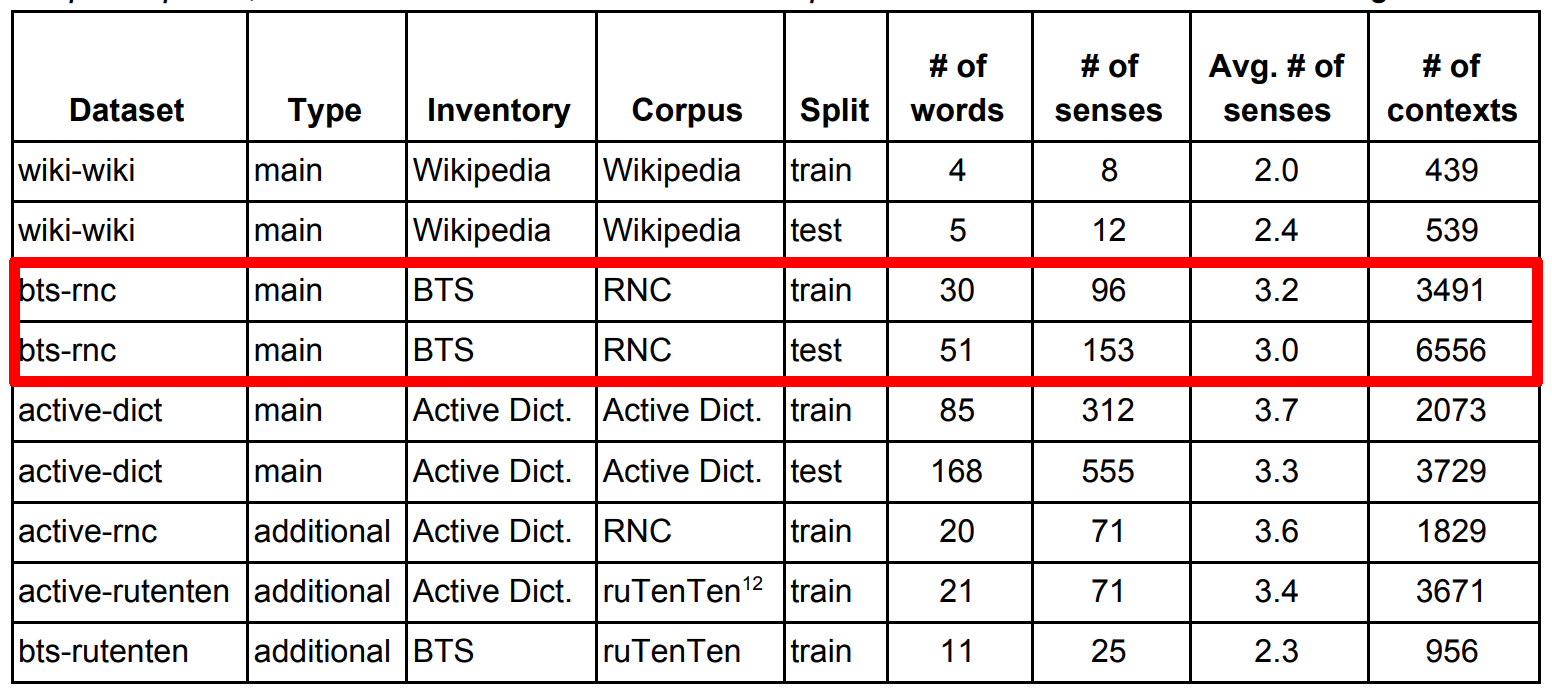
\includegraphics[width=1.0\textwidth]{figures/datasets2}
%}	
%\end{frame}
%
%
%\begin{frame}{Dataset based on dictionary glosses}
%
%{\centering
%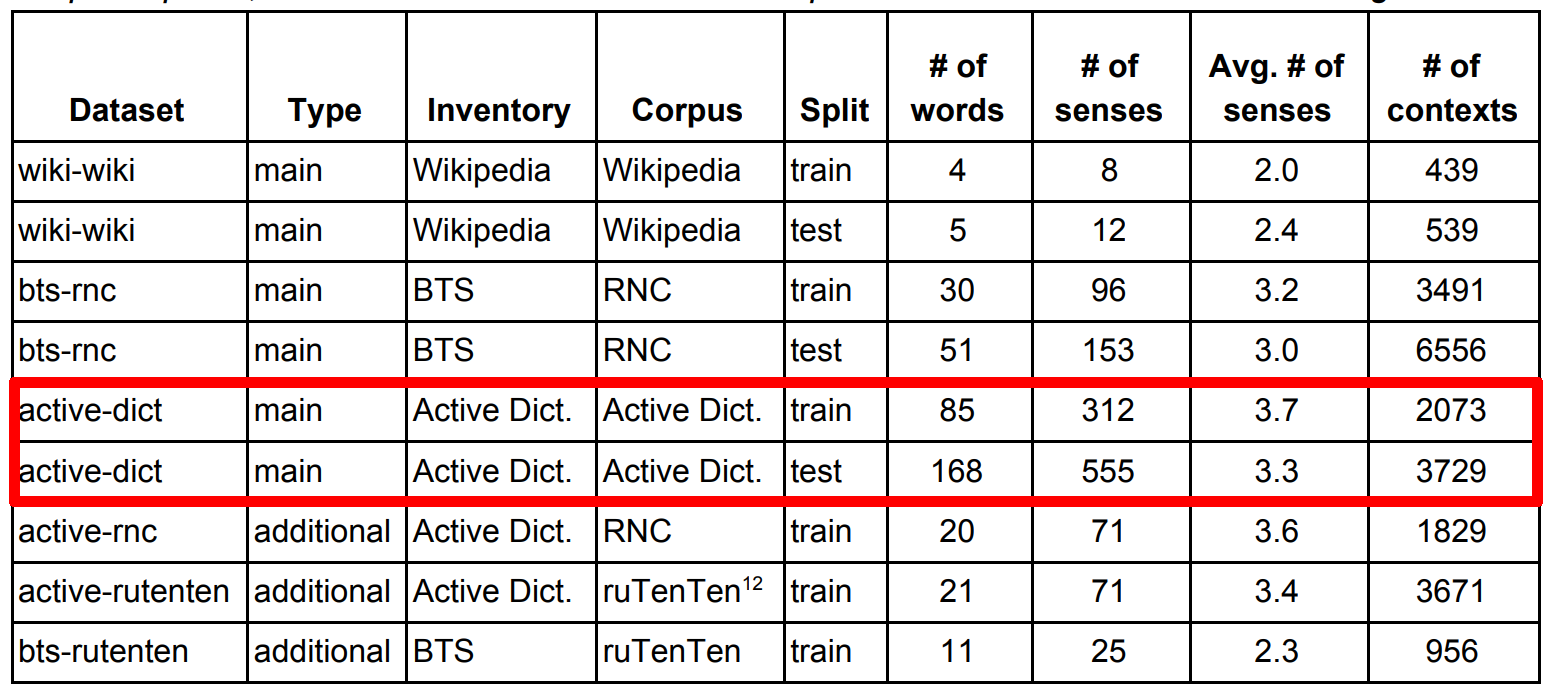
\includegraphics[width=1.0\textwidth]{figures/datasets3}
%}	
%\end{frame}
%
%
%
%\begin{frame}{A sample from the \textit{wiki-wiki} dataset }
%
%{\centering
%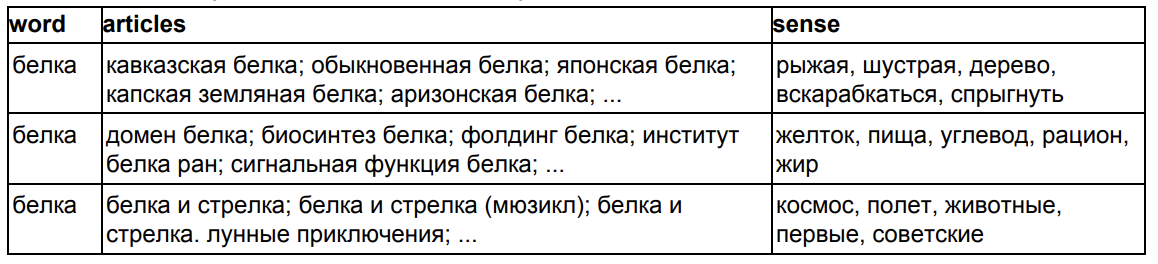
\includegraphics[width=1.0\textwidth]{figures/belka}
%}	
%\end{frame}
%
%
%
%\begin{frame}{A sample from the \textit{wiki-wiki} dataset }
%
%{\centering
%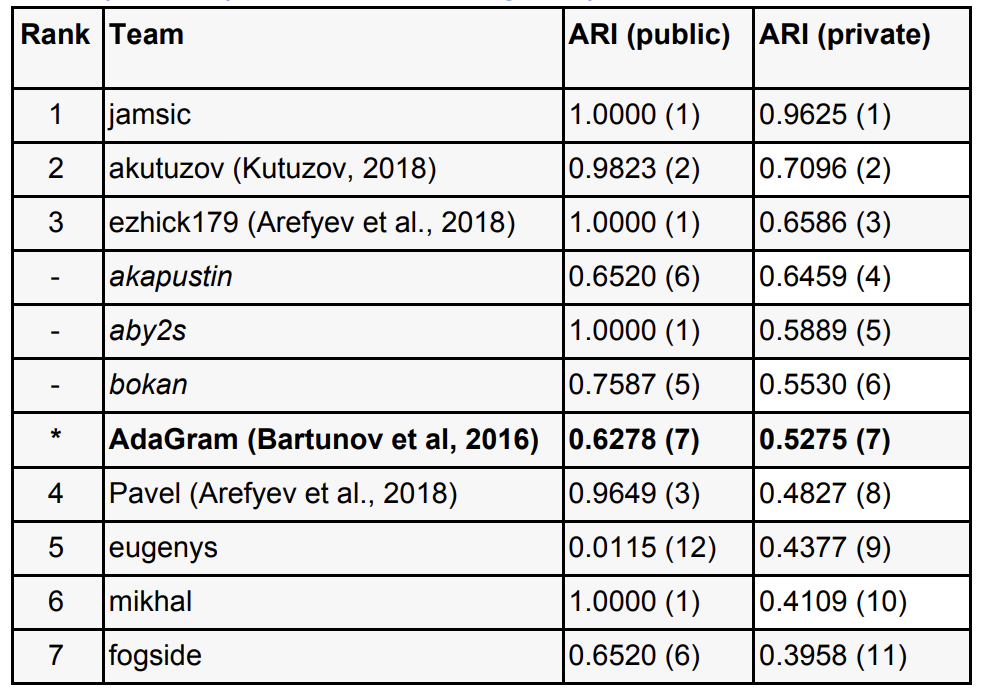
\includegraphics[width=.8\textwidth]{figures/wiki-wiki}
%}	
%\end{frame}
%
%
%
%\begin{frame}{A sample from the \textit{wiki-wiki} dataset }
%
%{\centering
%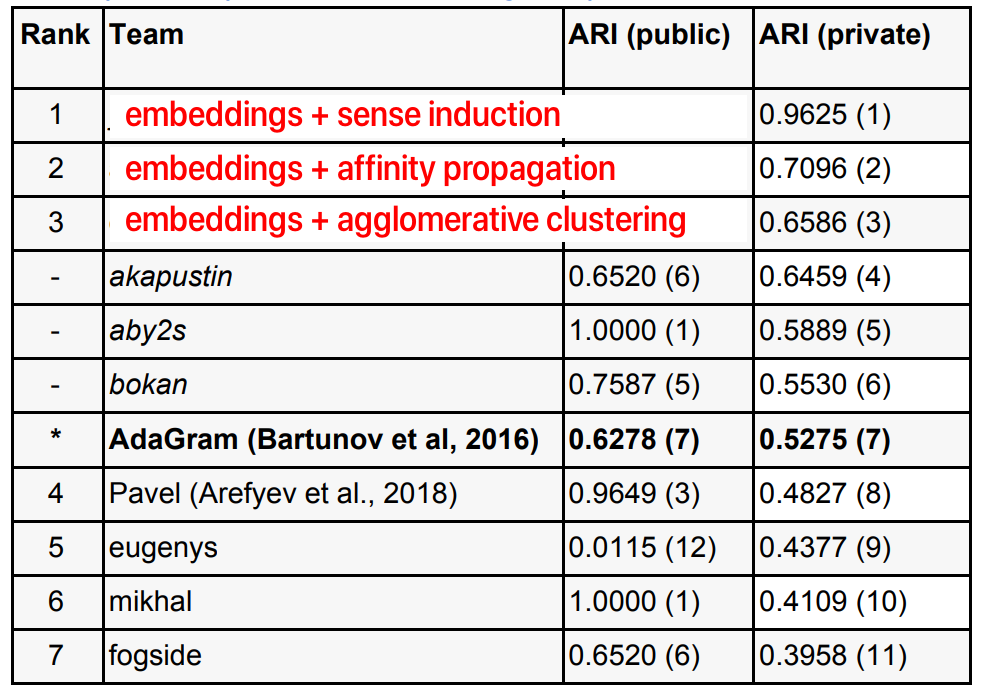
\includegraphics[width=.8\textwidth]{figures/wiki-wiki-top}
%}	
%\end{frame}
%
%
%
%\begin{frame}{A sample from the \textit{bts-rnc} dataset }
%
%{\centering
%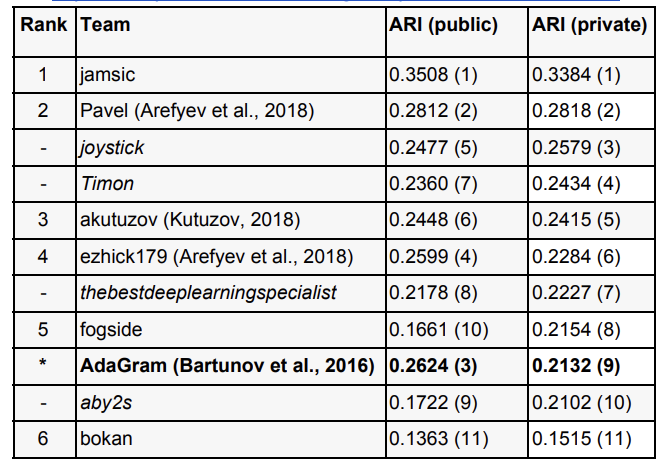
\includegraphics[width=.8\textwidth]{figures/bts}
%}	
%\end{frame}
%
%
%
%\begin{frame}{A sample from the \textit{active-dict} dataset }
%
%{\centering
%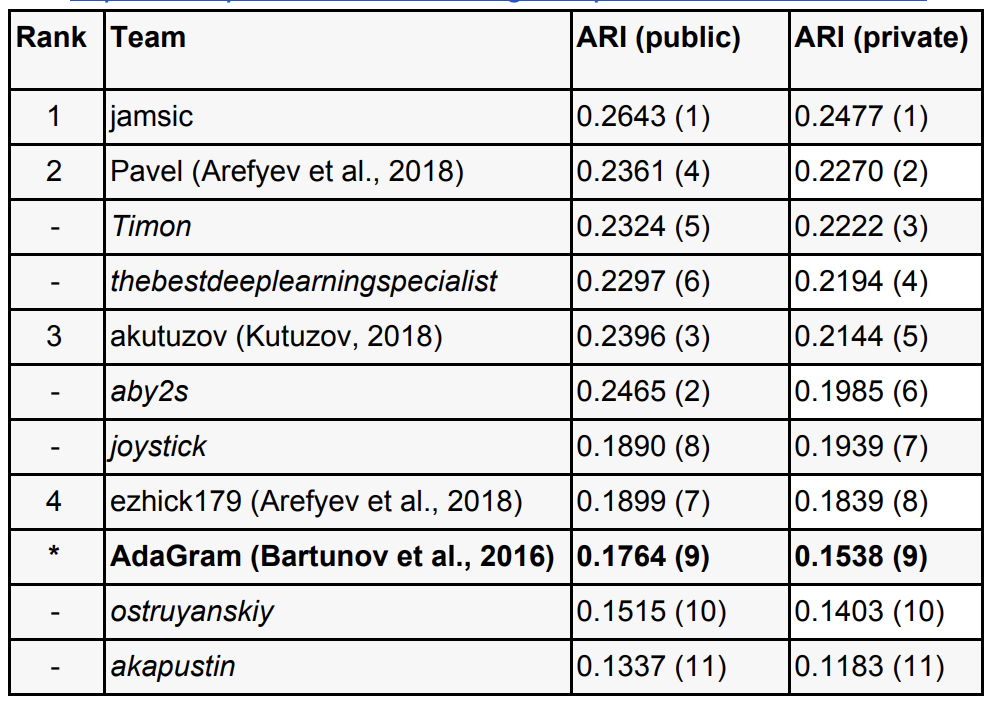
\includegraphics[width=.8\textwidth]{figures/active}
%}	
%\end{frame}



\begin{frame}{ Sense induction using clustering }


 \begin{center}
  	\includegraphics[width=0.99\textwidth]{figures/Clustering}
  \end{center}
  
  \pause 
  \begin{itemize}
  \item \textbf{\alert{Representation}}
  \begin{itemize}
  
  \item Sparse vector model (TF-IDF, etc.)
  \item Weighted (TF-IDF, $\chi^2$, etc.) sum of word embeddings
  \item Sentence embeddings (InterSent, Skip-Thougts, doc2vec, etc.)
  \end{itemize}
  
  \pause 
  \item \textbf{\alert{Clustering}}
  
  \begin{itemize}
  \item Affinity Propagation
  \item Agglomerative Clustering
  \item $k$-means
  \end{itemize} 	
  \end{itemize}


\end{frame}



\begin{frame}{ Sense induction using neighbors }

\begin{enumerate}
	\item \textbf{Get the neighbors} of a target word, e.g. \textbf{``bank''}:
	\begin{enumerate}
	\item \alert{lender}
	\item \textcolor{Cerulean}{river}
	\item \alert{citybank}
	\item \textcolor{Cerulean}{slope}
	\item ...
	\end{enumerate}
	
	\item Get \textbf{similar to ``bank''} and \textbf{dissimilar to \alert{``lender''}}:
	
	\begin{enumerate}
	\item \textcolor{Cerulean}{river}
	\item \textcolor{Cerulean}{slope}
	\item \textcolor{Cerulean}{land}
	\item ...
	\end{enumerate}
	 
\item \textbf{Compute distances} to \alert{\textbf{``lender''}} and \textcolor{Cerulean}{\textbf{``river''}}.
\end{enumerate}

\end{frame}





\begin{frame}{ Graph-vector sense induction }

\begin{enumerate}
\item \textbf{For} $i$-th neighbor of the target word $w$ among $k$ neigbours:

\begin{enumerate}
	\item Get a pair of opposite words for the $i$ neighbor: $(w_j, w_k)$
	\item Add them as as nodes: $V = V \cup \{w_j, w_k\}$
	\item Remember the pair as an anti-edge: $A = A \cup (w_j, w_k)$
\end{enumerate}

\pause 

\item \textbf{Build an ego network} $G = (V, E)$ of the word $w$:
\begin{enumerate}

\item $E$ are computed based on word similarities;
\item $E$ are pruned based on the anti-edge constraints: $E = E \smallsetminus
 A$.
	
\end{enumerate}

\pause 

\item \textbf{Cluster} the ego network of the word $w$.

\pause 

\item \textbf{Find cluster labels} by finding the central nodes in a cluster.

\end{enumerate}

\end{frame}






\begin{frame}{ Graph-vector sense induction }

\begin{itemize}
	\item \textbf{Get the neighbors} of a target word, e.g. \textbf{``java''}:
	\begin{enumerate}
	\item \alert{Python}
	\item \textcolor{Cerulean}{Borneo}
	\item \alert{C++}
	\item \textcolor{Cerulean}{Sumatra}
	\item \textcolor{Green}{Arabica}
    \item \textcolor{Green}{Robusta}
	\item \alert{Ruby}
	\item \alert{JavaScript}
	\item \textcolor{Cerulean}{Bali}

	\item ...
	\end{enumerate}

\end{itemize}

\end{frame}




\begin{frame}{ Graph-vector sense induction }

\begin{itemize}
	\item \textbf{Get the neighbors} of a target word, e.g. \textbf{``java''}:
	\begin{enumerate}
	\item \alert{Python} $\neq$ \textcolor{Cerulean}{Borneo}
	\item \textcolor{Cerulean}{Borneo} $\neq$ \alert{Scala}
	\item \alert{C++} $\neq$ \textcolor{Cerulean}{Borneo}
	\item \textcolor{Cerulean}{Sumatra} $\neq$ highway
	\item \textcolor{Green}{Arabica} $\neq$ \alert{Python}
    \item \textcolor{Green}{Robusta} $\neq$ \alert{Python}
	\item \alert{Ruby} $\neq$ \textcolor{Green}{Arabica}
	\item \textcolor{Cerulean}{Bali} $\neq$ North
	\end{enumerate}

\end{itemize}
\end{frame}




\begin{frame}{ Graph-vector sense induction }
\begin{itemize}

\item \textbf{Nodes}:

	\begin{enumerate}
	\item \alert{Python}
	\item \textcolor{Cerulean}{Borneo}
	\item \alert{C++}
	\item \textcolor{Green}{Arabica}
    \item \textcolor{Green}{Robusta}
	\item \alert{Ruby}
\end{enumerate}

\end{itemize}
\end{frame}





\begin{frame}{ Sense induction }


 \begin{center}
  	\includegraphics[height=0.69\textheight]{figures/bychok}
  \end{center}
  


\end{frame}




\begin{frame}{ Datasets }
\vspace{-10pt}

\begin{enumerate}
	\item SemEval 2007 
	\item SemEval 2010
	\item RUSSE 2018
	\item \textbf{SemEval 2019 Task 2 Subtask 1}:  
	\begin{itemize}
		\item Clustering of verb occurrences
		\item Assign occurrences of the target verbs to a number of clusters, in such a way that verbs belonging to the same cluster evoke the same frame type.
		\item gold annotations for this subtask are based on FrameNet
	\end{itemize}
	
\end{enumerate}

\pause 
\vspace{5pt}

\begin{itemize}
\footnotesize
\item Trump \textbf{leads} the world, backward.
\item Disrespecting international laws \textbf{leads} to many complications.
\item Rosenzweig \textbf{heads} the climate impacts section at NASA's Goddard Institute.
\end{itemize}

\end{frame}



\begin{frame}{ Datasets }
\vspace{-10pt}

\begin{enumerate}
	\item SemEval 2007 
	\item SemEval 2010
	\item RUSSE 2018
	\item \textbf{SemEval 2019 Task 2 Subtask 1}:  
	\begin{itemize}
		\item Clustering of verb occurrences
		\item Assign occurrences of the target verbs to a number of clusters, in such a way that verbs belonging to the same cluster evoke the same frame type.
		\item gold annotations for this subtask are based on FrameNet
	\end{itemize}
	
\end{enumerate}


\vspace{5pt}

\begin{itemize}
\footnotesize
\item \alert{Trump \textbf{leads} the world, backward.}
\item \textcolor{Cerulean}{Disrespecting international laws \textbf{leads} to many complications.}
\item \alert{Rosenzweig \textbf{heads} the climate impacts section at NASA's Goddard Institute.}
\end{itemize}

\end{frame}



\section{Induction of semantic frames}

\subsection{}

\begin{frame}{FrameNet: frame ``Kidnapping''}

\begin{center}	
\includegraphics[width=1.0\textwidth]{figures/fn-kidnap}
\end{center}

\end{frame}



\begin{frame}{Frame induction as a triclustering}

\begin{itemize}
\item \textbf{ACL'2018}~\cite{ustalov2018unsupervised}	
\end{itemize}

Example of a LU tricluster corresponding to the ``Kidnapping'' frame from FrameNet.

\begin{table}[t]
\centering
\begin{tabular}{lll}
\textbf{FrameNet~~~~~~~} & \textbf{Role~~~~~~~~} & \textbf{Lexical Units (LU)} \\\toprule
\textit{Perpetrator} & Subject & kidnapper, alien, militant \\ \midrule
\textit{FEE}         & Verb    & snatch, kidnap, abduct \\ \midrule
\textit{Victim}      & Object  & son, people, soldier, child \\
\end{tabular}

\end{table}	

\end{frame}



\begin{frame}{\textit{Triframes} frame induction}

\vspace{-10pt}
\begin{algorithmic}
\REQUIRE{an embedding model $v \in V \rightarrow \vec{v} \in \mathbb{R}^d$,}
\REQUIRE{a set of SVO triples $T \subseteq V^3$,}
\REQUIRE{the number of nearest neighbors $k \in \mathbb{N}$,}
\REQUIRE{a graph clustering algorithm $\textsc{Cluster}$.}
\pause 
\ENSURE{a set of triframes $F$.}
\pause 
\STATE{$S \gets \{t \!\rightarrow \vec{t} \in \mathbb{R}^{3d} : t \in T\}$}
\STATE{$E \gets \{(t, t') \in T^2 : t' \in \NN^S_k(\vec{t}), t \neq t'\}$}
\STATE{$F \gets \emptyset$}
\FORALL{$C \in \textsc{Cluster}(T, E)$}
\STATE{$f_s \gets \{s \in V : (s, v, o) \in C\}$}
\STATE{$f_v \gets \{v \in V : (s, v, o) \in C\}$}
\STATE{$f_o \gets \{o \in V : (s, v, o) \in C\}$}
\STATE{$F \gets F \cup \{(f_s, f_v, f_o)\}$}
\ENDFOR
\RETURN{$F$}
\end{algorithmic}

	
\end{frame}



\begin{frame}{Evaluation datasets}


\begin{tabular}{lrrr}
\textbf{Dataset} & \textbf{\# instances} & \textbf{\# unique} & \textbf{\# clusters} \\\toprule
FrameNet Triples   & 99,744 & 94,170 & 383 \\
Poly. Verb Classes &    246 &    110 & 62 \\
\end{tabular}
	
\end{frame}


\begin{frame}{Evaluation settings}


\begin{tabular}{lrrr}
\textbf{Dataset} & \textbf{\# instances} & \textbf{\# unique} & \textbf{\# clusters} \\\toprule
\textbf{\alert{FrameNet Triples}}   & 99,744 & 94,170 & 383 \\
Poly. Verb Classes &    246 &    110 & 62 \\
\end{tabular}

\pause 

\vspace{20pt}
\textbf{Quality Measures:}

\begin{itemize}
\item $\nmpu$: normalized modified purity, 
\item $\nipu$: normalized inverse purity.	
\end{itemize}

	
\end{frame}



\begin{frame}{Results: comparison to state-of-art}

\begin{center}	
\includegraphics[width=1.0\textwidth]{figures/frames2}
\end{center}


F\textsubscript{1}-scores for \legend{ggplotverb}\,verbs, \legend{ggplotsubject}\,subjects, \legend{ggplotobject}\,objects, \legend{ggplotframe}\,frames

\end{frame}


\section{Graph embeddings}
\subsection{}

\begin{frame}{\alert{Text}: sparse symbolic representation}

\begin{center}
	\includegraphics[width=\textwidth]{figures/w2v}
\end{center}

\pause 

Image source: \url{https://www.tensorflow.org/tutorials/word2vec}
	
\end{frame}




\begin{frame}{\alert{Graph}: sparse symbolic representation}

\begin{center}
	\includegraphics[width=\textwidth]{figures/g2v}
\end{center}
	
\end{frame}


\begin{frame}{Embedding graph into a vector space}

From a \textbf{survey on graph embeddings}~\cite{hamilton2017representation}:

\begin{center}
	\includegraphics[width=\textwidth]{figures/ge-fig1}
\end{center}

	
\end{frame}



\begin{frame}{Learning with an ``autoencoder''}

From a \textbf{survey on graph embeddings}~\cite{hamilton2017representation}:

\begin{center}
	\includegraphics[width=\textwidth]{figures/ge-fig2}
\end{center}

	
\end{frame}




\begin{frame}{Some established approaches}

From a \textbf{survey on graph embeddings}~\cite{hamilton2017representation}:

\begin{center}
	\includegraphics[width=\textwidth]{figures/ge-fig3}
\end{center}

	
\end{frame}





\begin{frame}{Graph embeddings using similarities}

An submitted joint work with Andrei Kutuzov and Chris Biemann:


\begin{itemize}
\item Given a tree $(V, E)$

\item \alert{\textbf{Leackock-Chodorow (LCH)}} similarity measure:
$$
sim(v_i, v_j)= −\log\frac{shortest\_path\_distance(v_i, v_j) }{2h} 
$$

\pause 
\item \alert{\textbf{Jiang-Conrath (JCN)}} similarity measure:

$$
sim(v_i, v_j) = 2 \frac{\ln P_{\alert{lcs}}(v_i, v_j)}{\ln P(v_i) + \ln P(v_j)} 
$$
\end{itemize}
	
\end{frame}



\begin{frame}{Graph embeddings using similarities}


\textit{path2vec} (\url{arxiv.org/abs/1808.05611}): Approximating \alert{\textbf{Structural Node Similarities}} with \textbf{Node Embeddings}:

$$
J = \frac{1}{|T|}  \sum_{ (v_i, v_j) \in T }  (\mathbf{v}_i \cdot \mathbf{v}_j - sim(v_i, v_j) )^2,
$$

where:

\begin{itemize}
	\item $sim(v_i, v_j)$ - the value of a `gold' similarity measure between a pair of nodes $v_i$ and $v_j$;
	\item $\mathbf{v}_i$ - an embeddings of node;
	\item $T$ - training batch.
\end{itemize}

\end{frame}

\begin{frame}{Speedup: graph vs embeddings}	

Computation of 82,115 pairwise similarities:

\begin{table}
\begin{tabular}{lc}
\toprule
\textit{Model} & \textit{Running time} \\
\midrule
LCH in NLTK & 30 sec. \\
JCN in NLTK & 6.7 sec. \\
%\midrule
FSE embeddings & 0.713 sec. \\
%\midrule
\textit{path2vec} and other float vectors & \textbf{0.007} sec. \\
\bottomrule
\end{tabular}
\end{table}

\end{frame}


\begin{frame}{Results: goodness of fit}


\textbf{Spearman correlation scores with WordNet similarities on SimLex999 noun pairs}:

\begin{table}
\begin{tabular}{lccc}
\toprule
& \multicolumn{3}{c}{\textit{Selection of synsets}} \\
Model & JCN-SemCor & JCN-Brown & LCH \\
\midrule
WordNet & 1.0  & 1.0  & 1.0  \\
\midrule
Node2vec & 0.655 & 0.671 & 0.724  \\
Deepwalk & 0.775 & 0.774  & 0.868 \\
FSE & 0.830  & 0.820 & 0.900  \\
\midrule
path2vec & \textbf{0.917}  & \textbf{0.914}  & \textbf{0.934}  \\
\bottomrule
\end{tabular}
\end{table}

\end{frame}




\begin{frame}{Results: SimLex999 dataset}


\textbf{Spearman correlations with human SimLex999 noun similarities:}


\begin{table}
\begin{tabular}{lc}
\toprule
\textit{Model} & \textit{Correlation} \\
\midrule
Raw WordNet JCN-SemCor & 0.487  \\
Raw WordNet JCN-Brown & 0.495  \\
Raw WordNet LCH & 0.513  \\
\midrule
node2vec { \cite{grover2016node2vec}} & 0.450  \\
Deepwalk { \cite{perozzi2014deepwalk}} & 0.533  \\
FSE { \cite{subercaze:2015}} & \textbf{0.556}  \\
path2vec JCN-SemCor & 0.526  \\
path2vec JCN-Brown & 0.487  \\
path2vec LCH & 0.522  \\
\bottomrule
\end{tabular}
\end{table}

\end{frame}



\begin{frame}{Results: SimLex999 dataset}

\textbf{JCN (left) and LCH (right)}:

\begin{figure}
    \centering
    \includegraphics[width=0.49\textwidth]{figures/jcn-semcor-thresh01-near50_dynamic_synsets.png}
     \includegraphics[width=0.49\textwidth]{figures/lch-thresh15-near50_dynamic_synsets.png}
       
\end{figure}
	
\end{frame}


\begin{frame}{Results: word sense disambiguation}

\textbf{WSD: each column lists all the possible synsets for the corresponding word.}


\begin{figure}
       \centering
       \includegraphics[width=\textwidth]{figures/graph_wsd_example}
\end{figure}
	
\end{frame}


\begin{frame}{Results: word sense disambiguation}

\textbf{F1 scores on Senseval-2 word sense disambiguation task}:

\begin{table}
\footnotesize
\begin{tabular}{lccc}
\toprule
Model & \multicolumn{3}{c}{F-measure} \\
\midrule
WordNet JCN-SemCor & \multicolumn{3}{c}{\textbf{0.620}} \\
WordNet JCN-Brown &   \multicolumn{3}{c}{0.561} \\
WordNet LCH & \multicolumn{3}{c}{0.547} \\
node2vec~\cite{grover2016node2vec} & \multicolumn{3}{c}{0.501} \\
Deepwalk~\cite{perozzi2014deepwalk} & \multicolumn{3}{c}{0.528} \\
FSE~\cite{subercaze:2015}  & \multicolumn{3}{c}{0.536} \\
\midrule
\multicolumn{4}{c}{ \textit{path2vec}} \\
\midrule
\textit{Batch size:} & 20 & 50 & 100 \\
\midrule
JCN-SemCor & \textbf{0.543} & \textbf{0.543} & 0.535 \\
JCN-Brown & 0.538 & 0.515 & 0.542 \\
LCH & 0.540 & 0.535 & 0.536 \\
\bottomrule
\end{tabular}
\end{table}
	
\end{frame}




\begin{frame}{Improved Model and Results}

%
%Original model:
%$$
%\mathcal{L} = \frac{1}{|T|}  \sum_{ (v_i, v_j) \in T }  (\mathbf{v}_i \cdot \mathbf{v}_j - sim(v_i, v_j) )^2,
%$$
%
%
%Improved model:
$$
\mathcal{L} = \frac{1}{|T|}  \sum_{ (v_i, v_j) \in T } \left( (\mathbf{v}_i \cdot \mathbf{v}_j - sim(v_i, v_j) )^2  + \alert{\mathbf{v}_i \cdot \mathbf{v}_{in}} + \alert{\mathbf{v}_j \cdot \mathbf{v}_{jm}} \right) ,
$$


where:

\begin{itemize}
	\item $sim(v_i, v_j)$ - the value of a `gold' similarity measure between a pair of nodes $v_i$ and $v_j$;
	\item $\mathbf{v}_i$ - an embeddings of node;
	\item $T$ - training batch; 
	\item \alert{$v_{in}$ - random adjacent node of $v_i$}.
\end{itemize}

\end{frame}




\section{Conclusion}

%
%\begin{frame}{Vectors + Graphs = $\heartsuit$ }
%
%\begin{center}
%\includegraphics[width=0.7\textwidth]{figures/graphs}	
%\end{center}
%
%\end{frame}

\begin{frame}{Take home messages}

\vspace{-10pt}

\begin{itemize}
	\item We can \alert{\textbf{induce word senses}}, \alert{\textbf{synsets}}, \alert{\textbf{semantic classes}}, and \textbf{\alert{semantic frames}} in a knowledge-free way using \textbf{graph clustering} and \textbf{distributional models}.
    \vspace{1em}
    \pause
    
	\item We can make the \alert{\textbf{induced word senses interpretable}} in a knowledge-free way with \textbf{hypernyms}, \textbf{images},  \textbf{definitions}. 
	\vspace{1em}
    \pause
	
	\item We can \alert{\textbf{link induced senses to lexical resources}} to
	\begin{itemize} 
		\item improve \textbf{performance of WSD};
		\item \textbf{enrich lexical resources} with emerging senses;
		\item See~\cite{panchenko2016best,faralli2016linked,panchenko-EtAl:2017:SENSE2017,biemann2018framework}
	\end{itemize}
	
	\pause 
	\item We can \textbf{\alert{represent language graphs}} using graph embeddings for  use in \textbf{deep neural models}.
	
\end{itemize}


\end{frame}

%
%\begin{frame}{Natural Language Engineering journal}
%
%\vspace{-8pt} 
%\begin{itemize}
%\item A special issue on \textbf{\alert{informing neural architectures for NLP with linguistic and background knowledge}}.
%\item ... with \textbf{Ivan Vuli\'c} and \textbf{Simone Paolo Ponzetto}. 
% \end{itemize}
%
%\begin{center}
%	\includegraphics[width=.2\textwidth]{figures/nle-journal}
%	\includegraphics[width=.63\textwidth]{figures/cambridge-core}
%\end{center}
%
%\textbf{\LARGE \alert{\url{goo.gl/A76NGX}}}
%	
%	
%\end{frame}


%\begin{frame}{\alert{\textbf{Thank you! Questions?}} }
%
%  \animategraphics[loop,autoplay,width=\linewidth]{2}{figures/he}{1}{4}
%
%%\includegraphics[width=0.25\textwidth]{figures/dfg} \includegraphics[width=0.15\textwidth]{figures/daad}
%
%\end{frame}




\bibliography{biblio}
\bibliographystyle{apalike2}


\end{document}

